\subsubsection{Trang Đích}
Giao diện trang đích sẽ được hiển thị với mọi người dùng. Nội dung sẽ hiển thị các thông tin quan trọng và cần thiết nhất của của hệ thống, giúp người dùng hình dung được giá trị mà hệ thống mang lại. Trang đích gồm có trang chính hình 71 và trang giới thiệu hình 72. Trang chính chứa màn hình chào, các tính năng nổi bật, các gói dịch vụ, cách hoạt động và đăng ký ngay. Trang giới thiệu chứa thông tin công ty, sứ mệnh và đội ngũ. Ngoài ra còn có thanh header chứa logo, các nút điều hướng và thanh footer chứa các thông tin liên hệ.
\begin{figure}[H]
	\centering
	\fbox{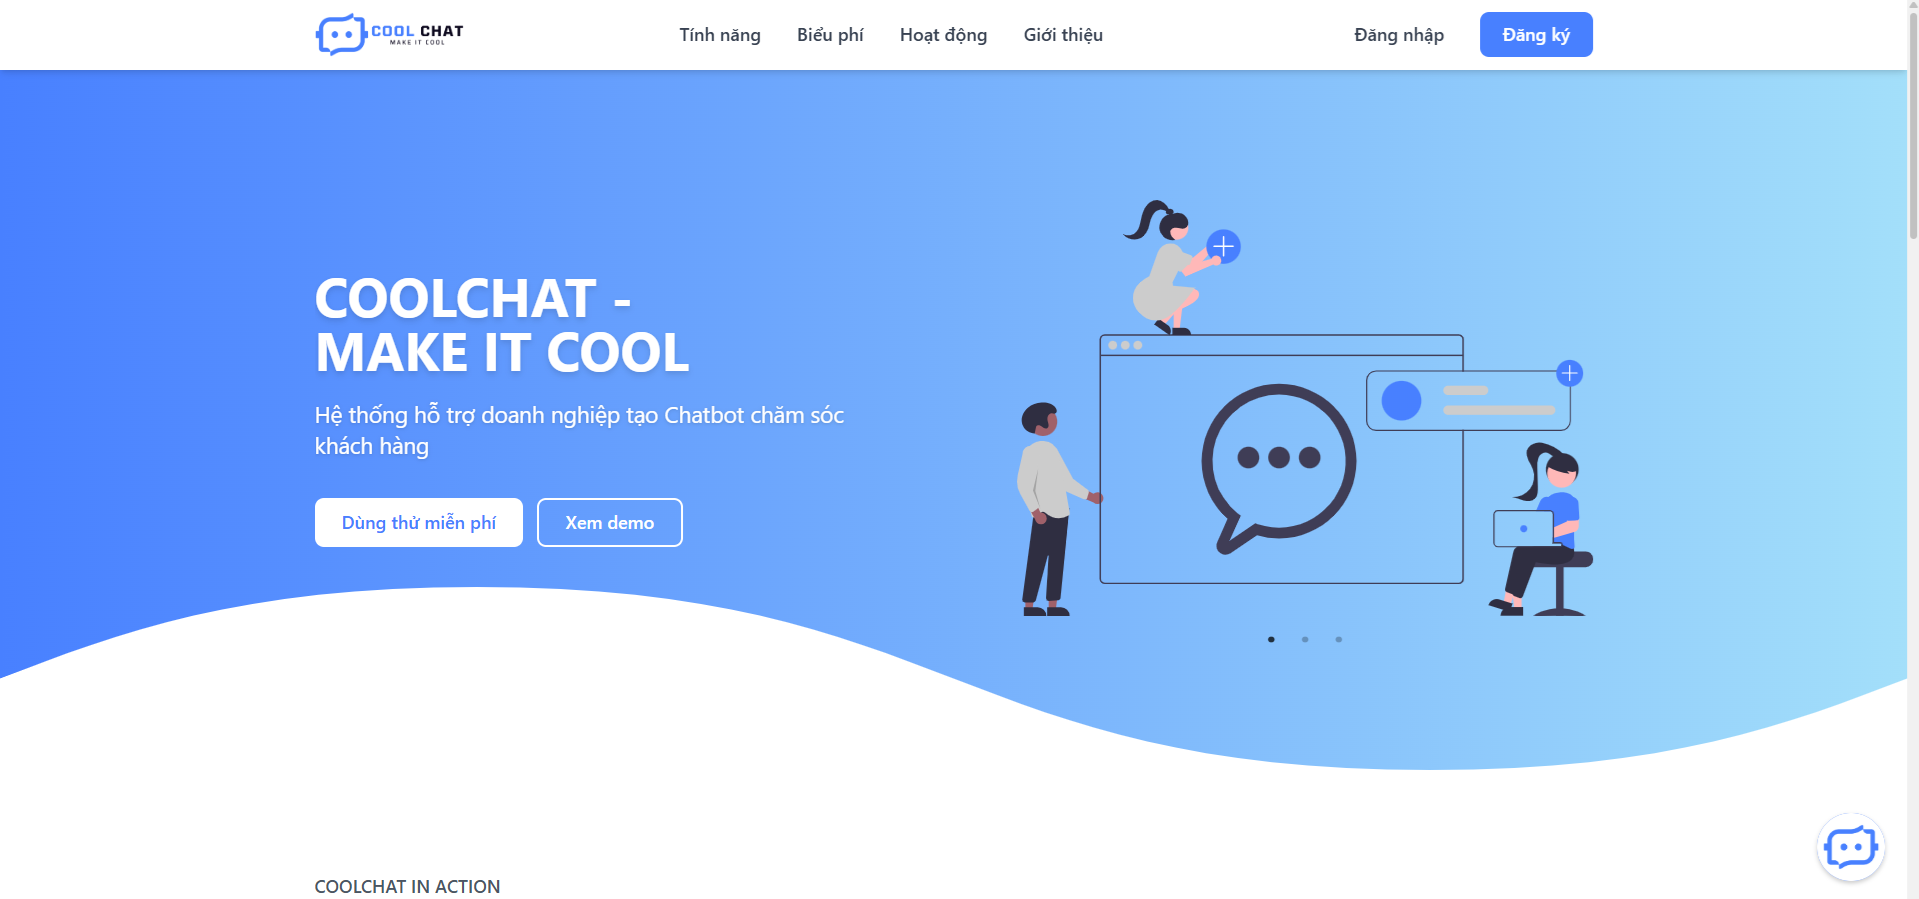
\includegraphics[width=1\textwidth]{Figma/landing_imple_1.png}}
	\vspace{0.5cm}
	\caption{Giao diện trang đích chính}
	\label{fig:enter-label}
\end{figure}
\begin{figure}[H]
	\centering
	\fbox{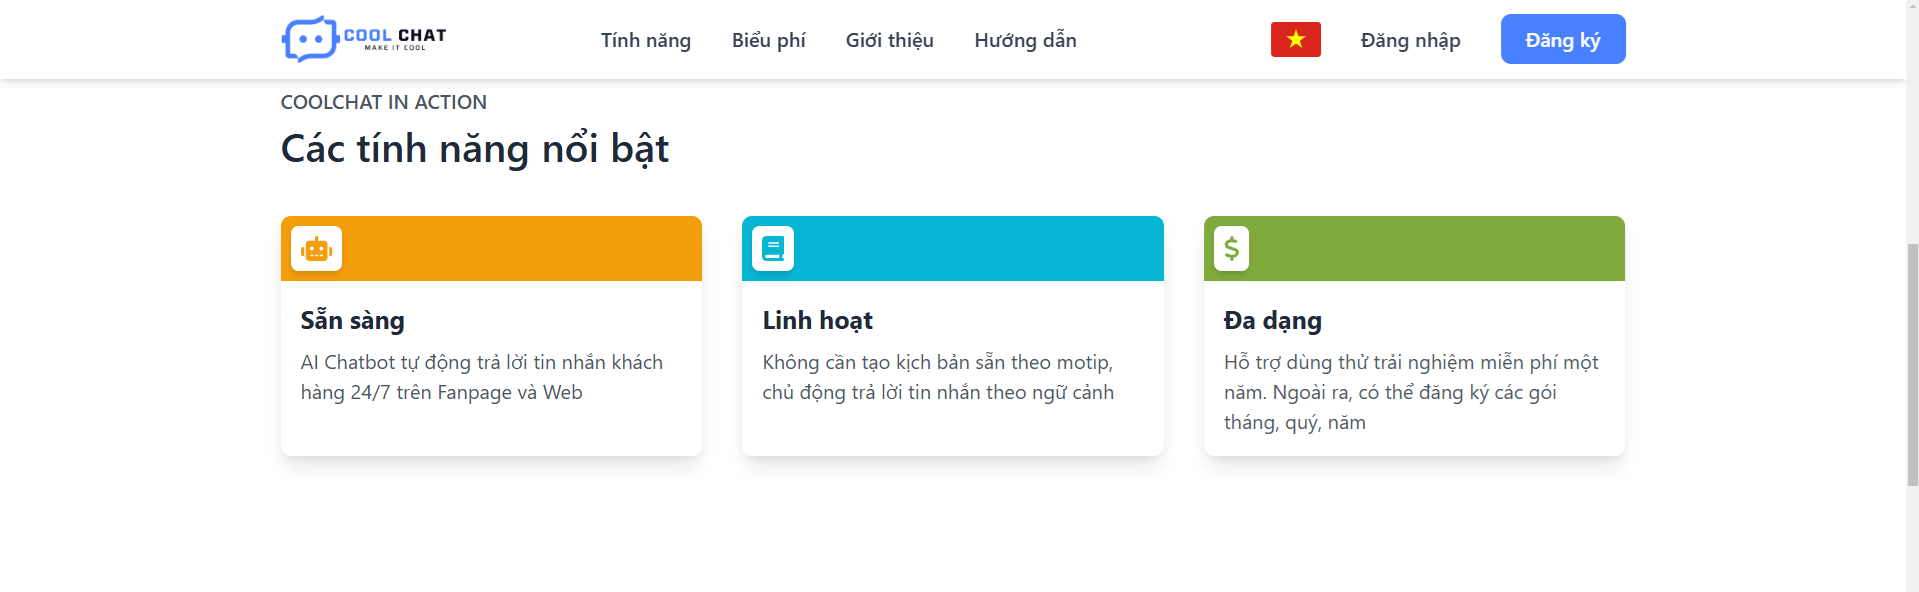
\includegraphics[width=1\textwidth]{Figma/landing_imple_2.png}}
	\vspace{0.5cm}
	\caption{Giao diện trang giới thiệu}
	\label{fig:enter-label}
\end{figure}
\subsubsection{Trang Xác thực}
Hệ thống sẽ cung cấp các chức năng xác thực như đăng nhập, tạo tổ chức, tham gia tổ chức, quên mật khẩu cho ba loại người dùng là chủ sở hữu tổ chức, quản trị viên tổ chức và nhân viên chăm sóc khách hàng. Hình 73 là giao diện trang đăng nhập của hệ thống.
\begin{figure}[H]
	\centering
	\fbox{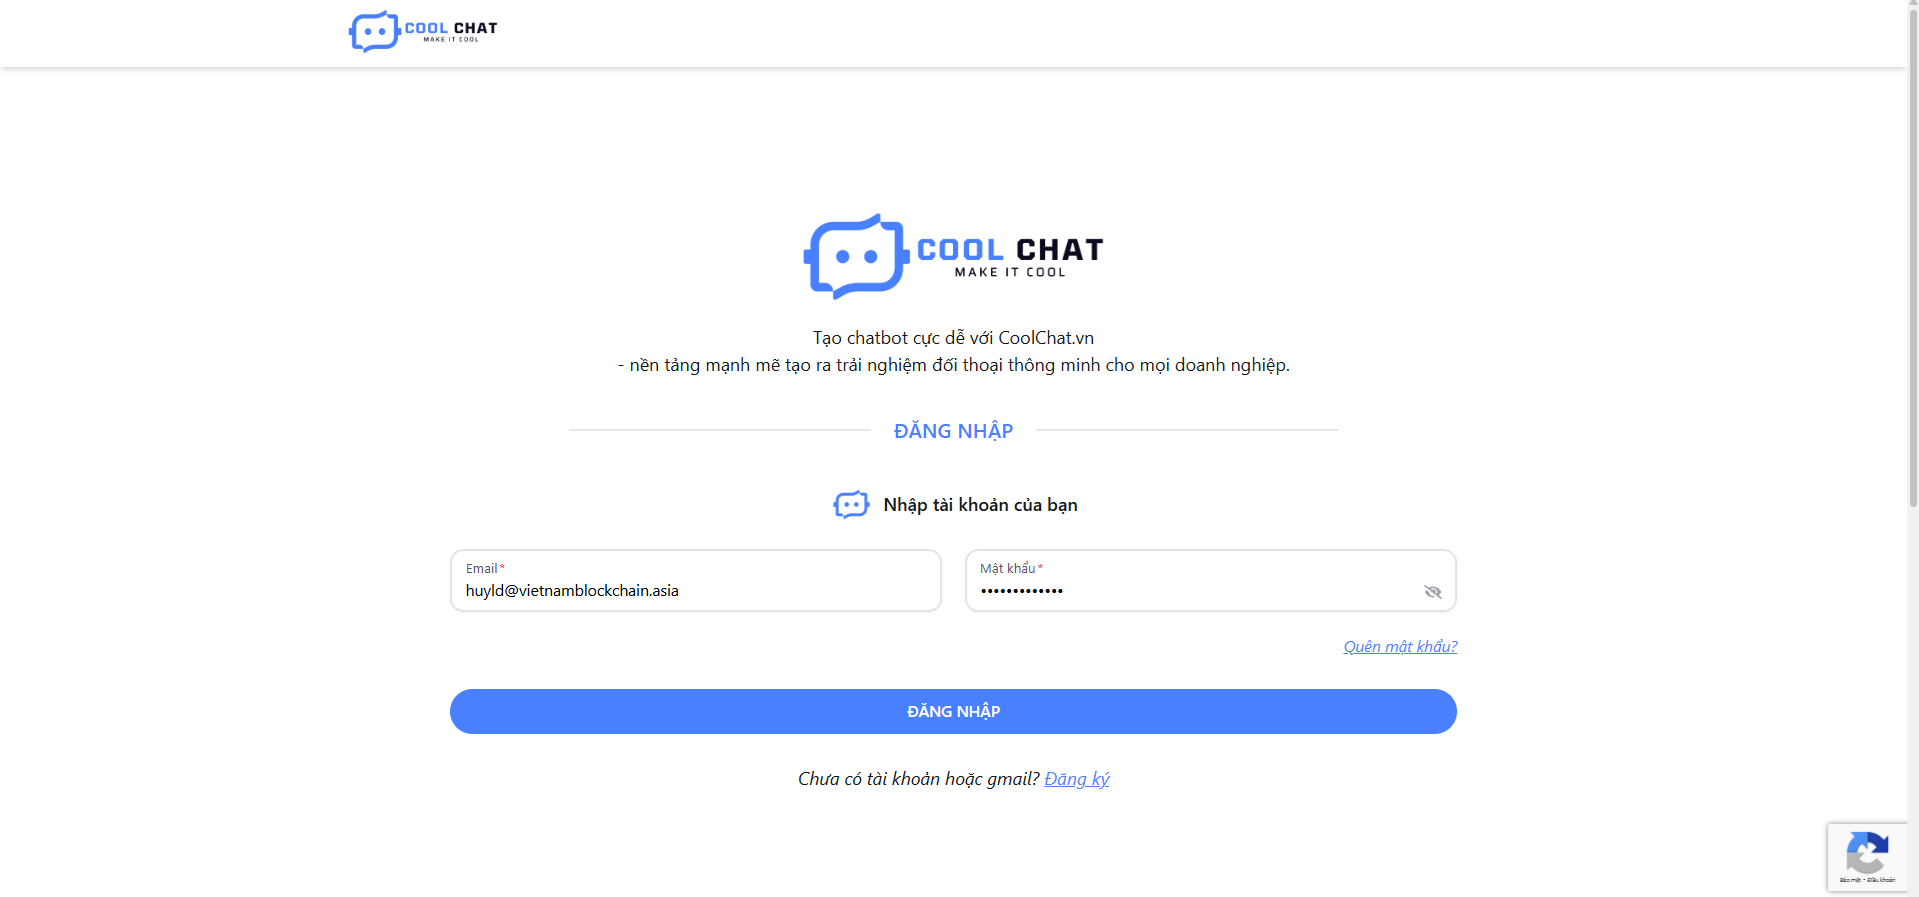
\includegraphics[width=0.9\textwidth]{Figma/login_imple.png}}
	\vspace{0.5cm}
	\caption{Giao diện đăng nhập}
	\label{fig:enter-label}
\end{figure}

Đối với giao diện đăng ký ở hình 74, người dùng có thể chọn tạo một tổ chức mới hoặc tham gia một tổ chức đã tồn tại sử dụng mã giới thiệu được gửi qua địa chỉ email.
\begin{figure}[H]
	\centering
	\fbox{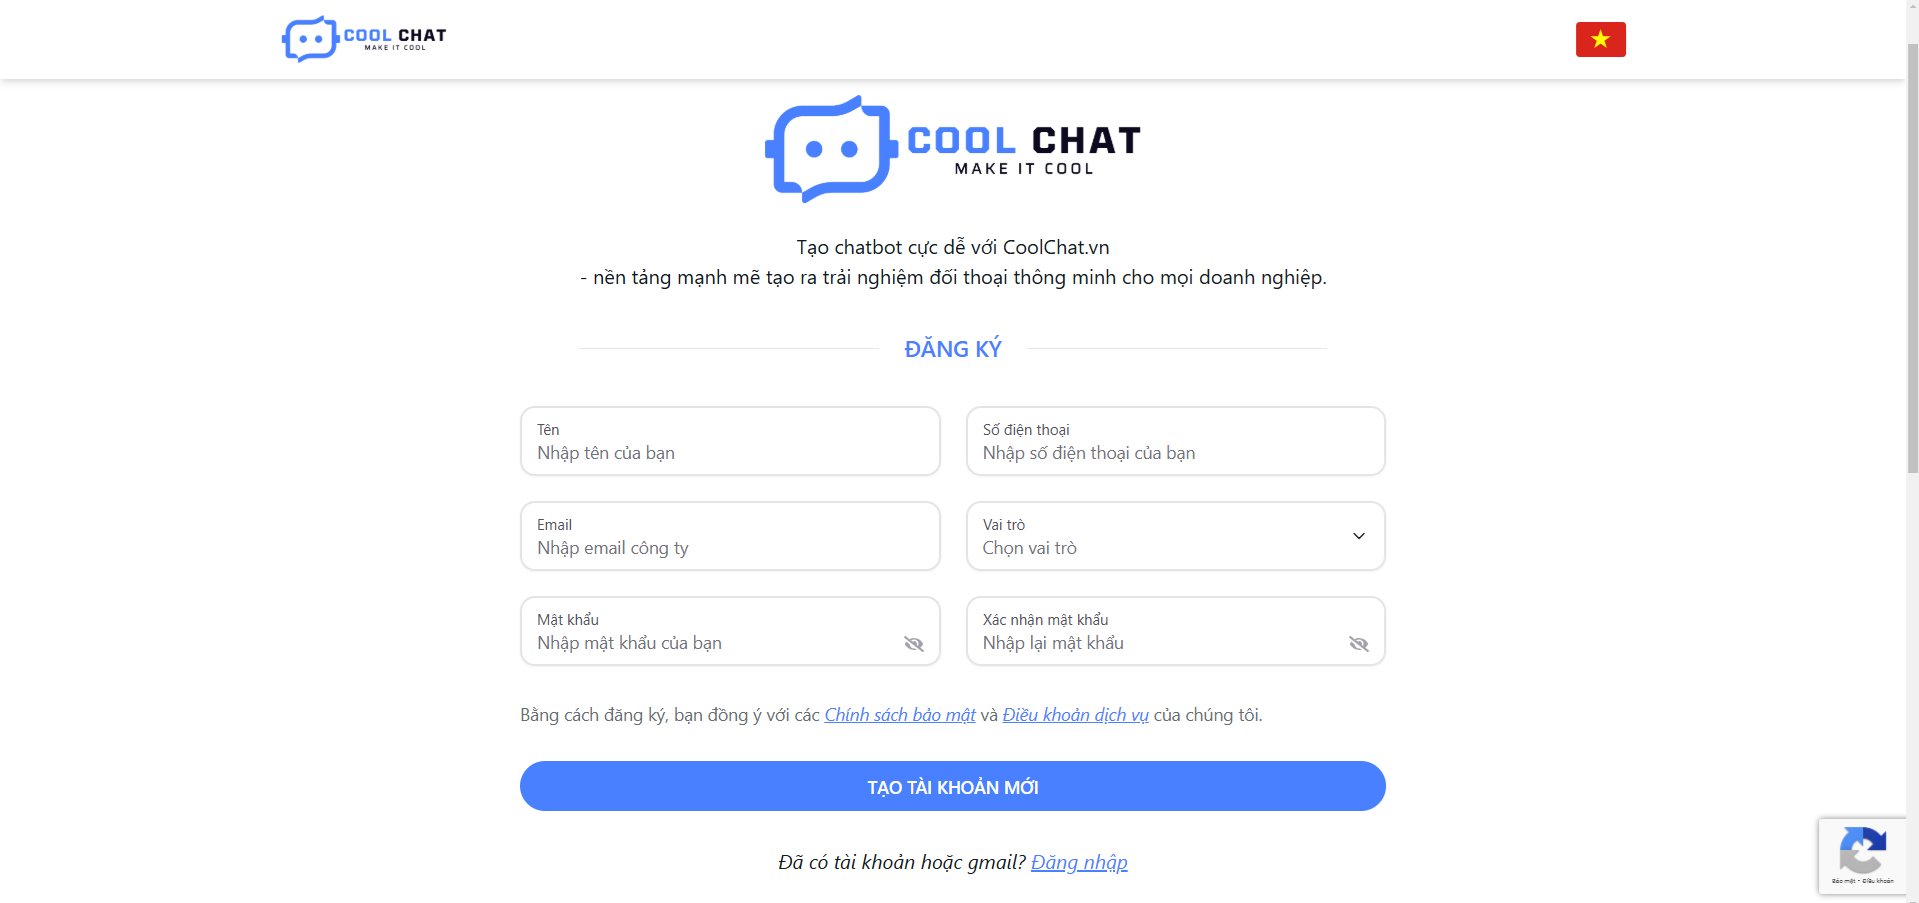
\includegraphics[width=0.9\textwidth]{Figma/signup_imple.png}}
	\vspace{0.5cm}
	\caption{Giao diện đăng ký}
	\label{fig:enter-label}
\end{figure}

Khi người dùng tạo tổ chức, được mời tham gia tổ chức, quên mật khẩu, người dùng sẽ nhận được một địa chỉ email để xác minh tương tự như hình 75.
\begin{figure}[H]
	\centering
	\fbox{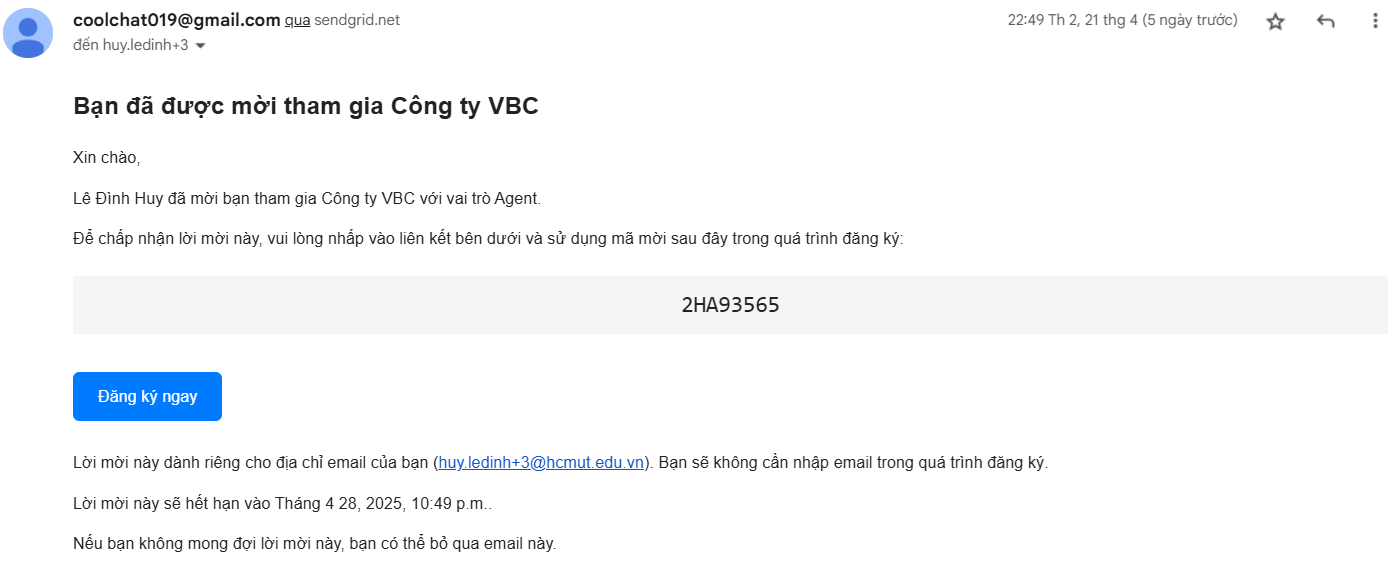
\includegraphics[width=0.9\textwidth]{Figma/signup_imple_create_email.png}}
	\vspace{0.5cm}
	\caption{Email tham gia tổ chức được gửi bởi hệ thống}
	\label{fig:enter-label}
\end{figure}

Mỗi trang đều chứa đầy đủ các thành phần cần thiết, bố cục hài hòa, màu sắc bắt mắt.

\subsubsection{Trang Đào tạo chatbot}
Sau khi đăng nhập thành công với vai trò Chủ sở hữu/Quản trị viên, người dùng sẽ vào trang Đào tạo chatbot như hình 76. Trang gồm có mục quản lý tri thức và mục cập nhật tri thức.

Đối với quản lý tri thức, người dùng quan sát thấy một danh sách các tri thức hiện có với các thông tin của từng tri thức. Người dùng có thể tìm kiếm, lọc, xem trang, chỉnh sửa, xem chi tiết, tải xuống, xóa và nhấn nút lưu và đào tạo tri thức.
\begin{figure}[H]
	\centering
	\fbox{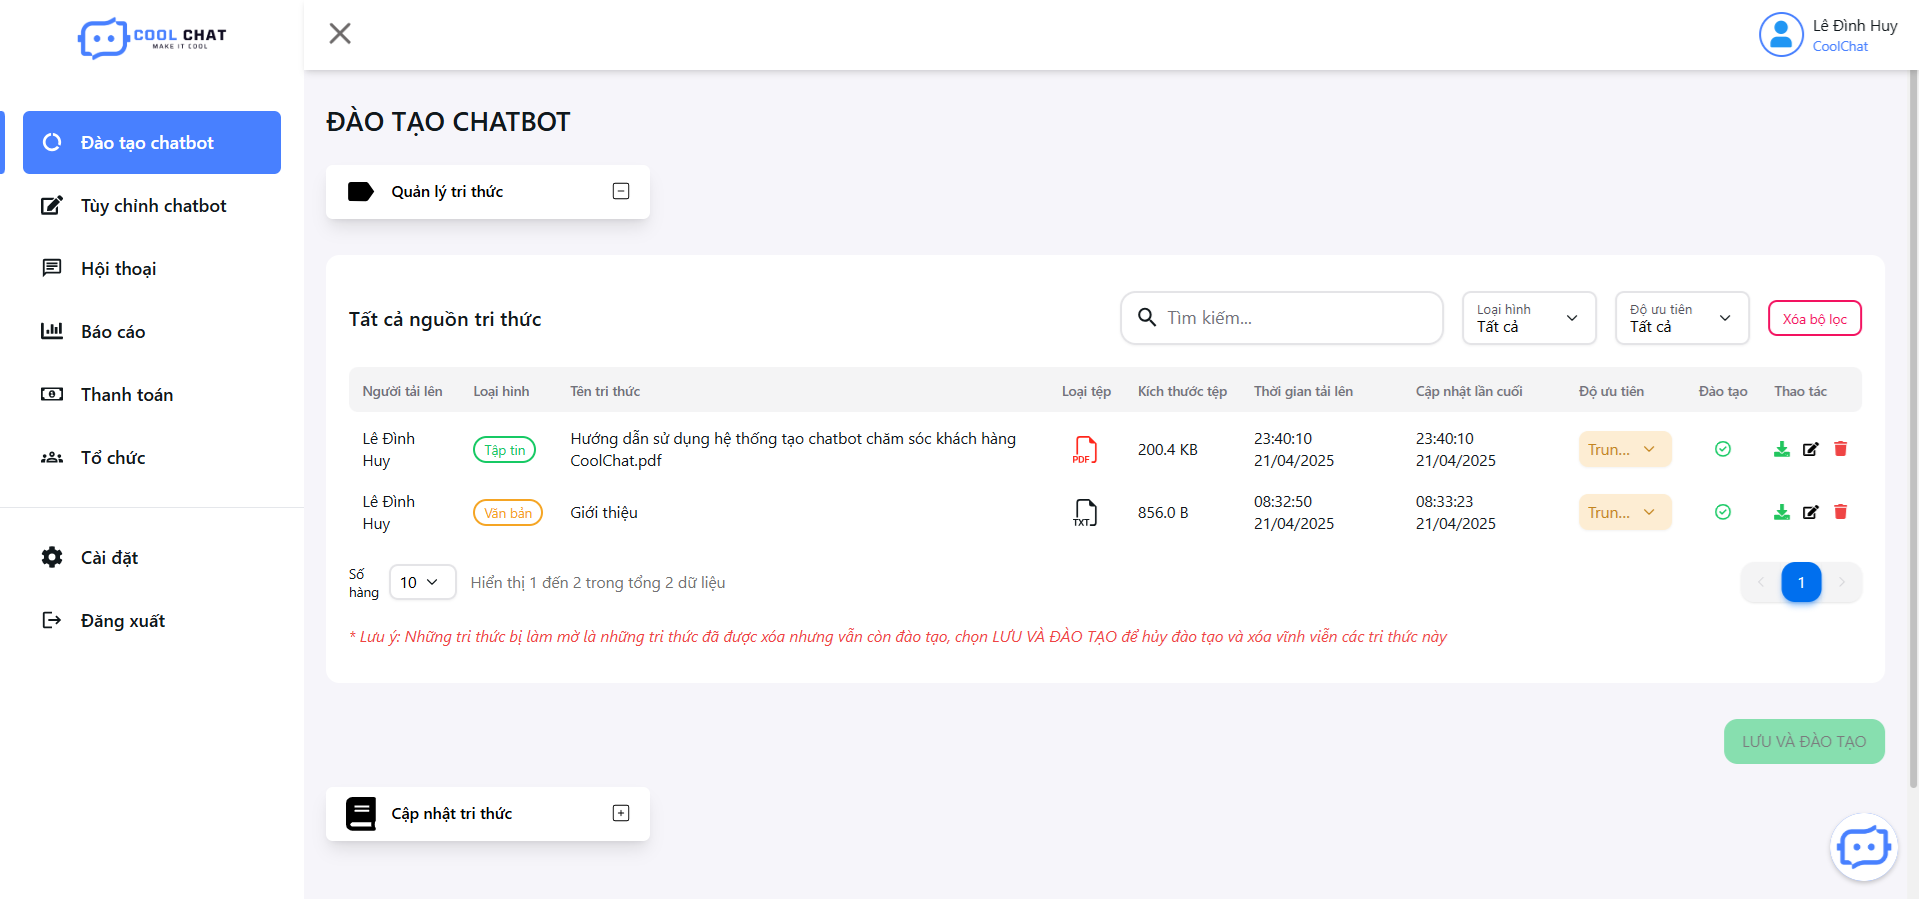
\includegraphics[width=1\textwidth]{Figma/chatbottraining_imple.png}}
	\vspace{0.5cm}
	\caption{Giao diện mục Quản lý tri thức}
	\label{fig:enter-label}
\end{figure}

Khi bấm tải xuống một tri thức có dạng tập tin hoặc văn bản, hệ thống sẽ hiện thị bản xem trước cho tri thức có loại tệp .txt và .pdf như hình 77, loại tệp .docx sẽ được tải ngay xuống thiết bị của người dùng.
\begin{figure}[H]
	\centering
	\fbox{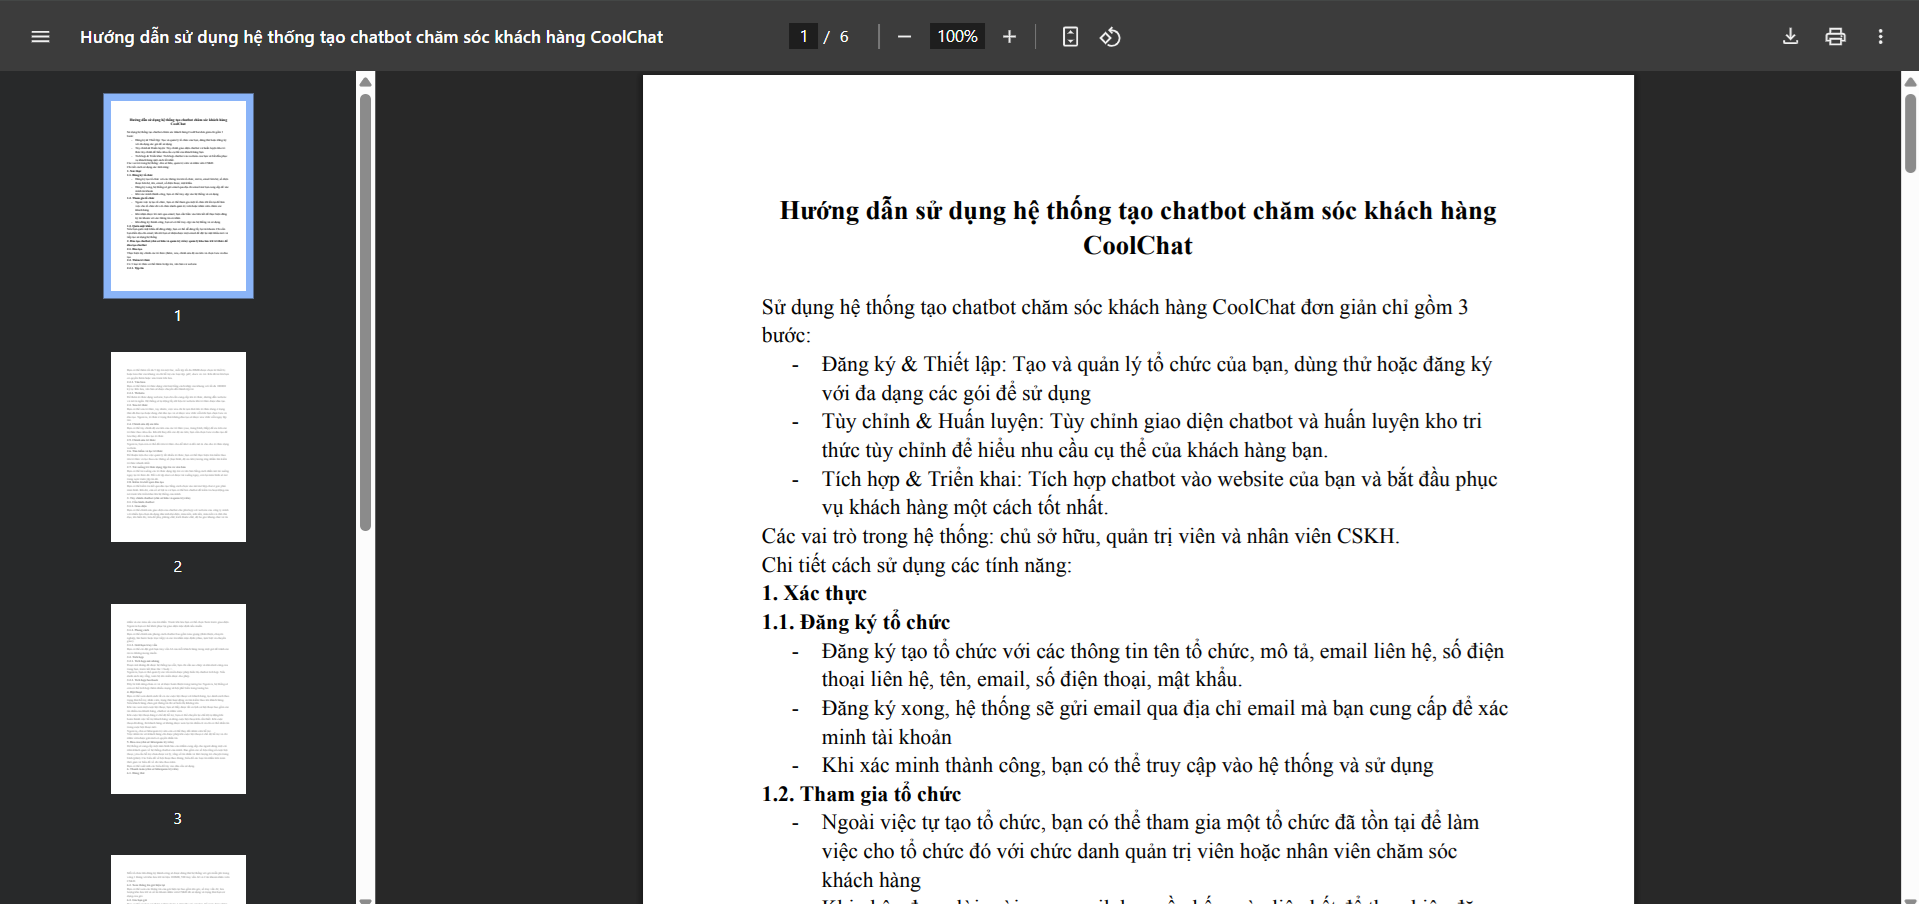
\includegraphics[width=1\textwidth]{Figma/download.png}}
	\vspace{0.5cm}
	\caption{Bản xem trước khi tải xuống tri thức}
	\label{fig:enter-label}
\end{figure}


Đối với cập nhật tri thức, người dùng có thể chọn một trong ba loại tập tin, văn bản hoặc website để thêm tri thức mới như ở hình 78, 79 và 80.
\begin{figure}[H]
	\centering
	\fbox{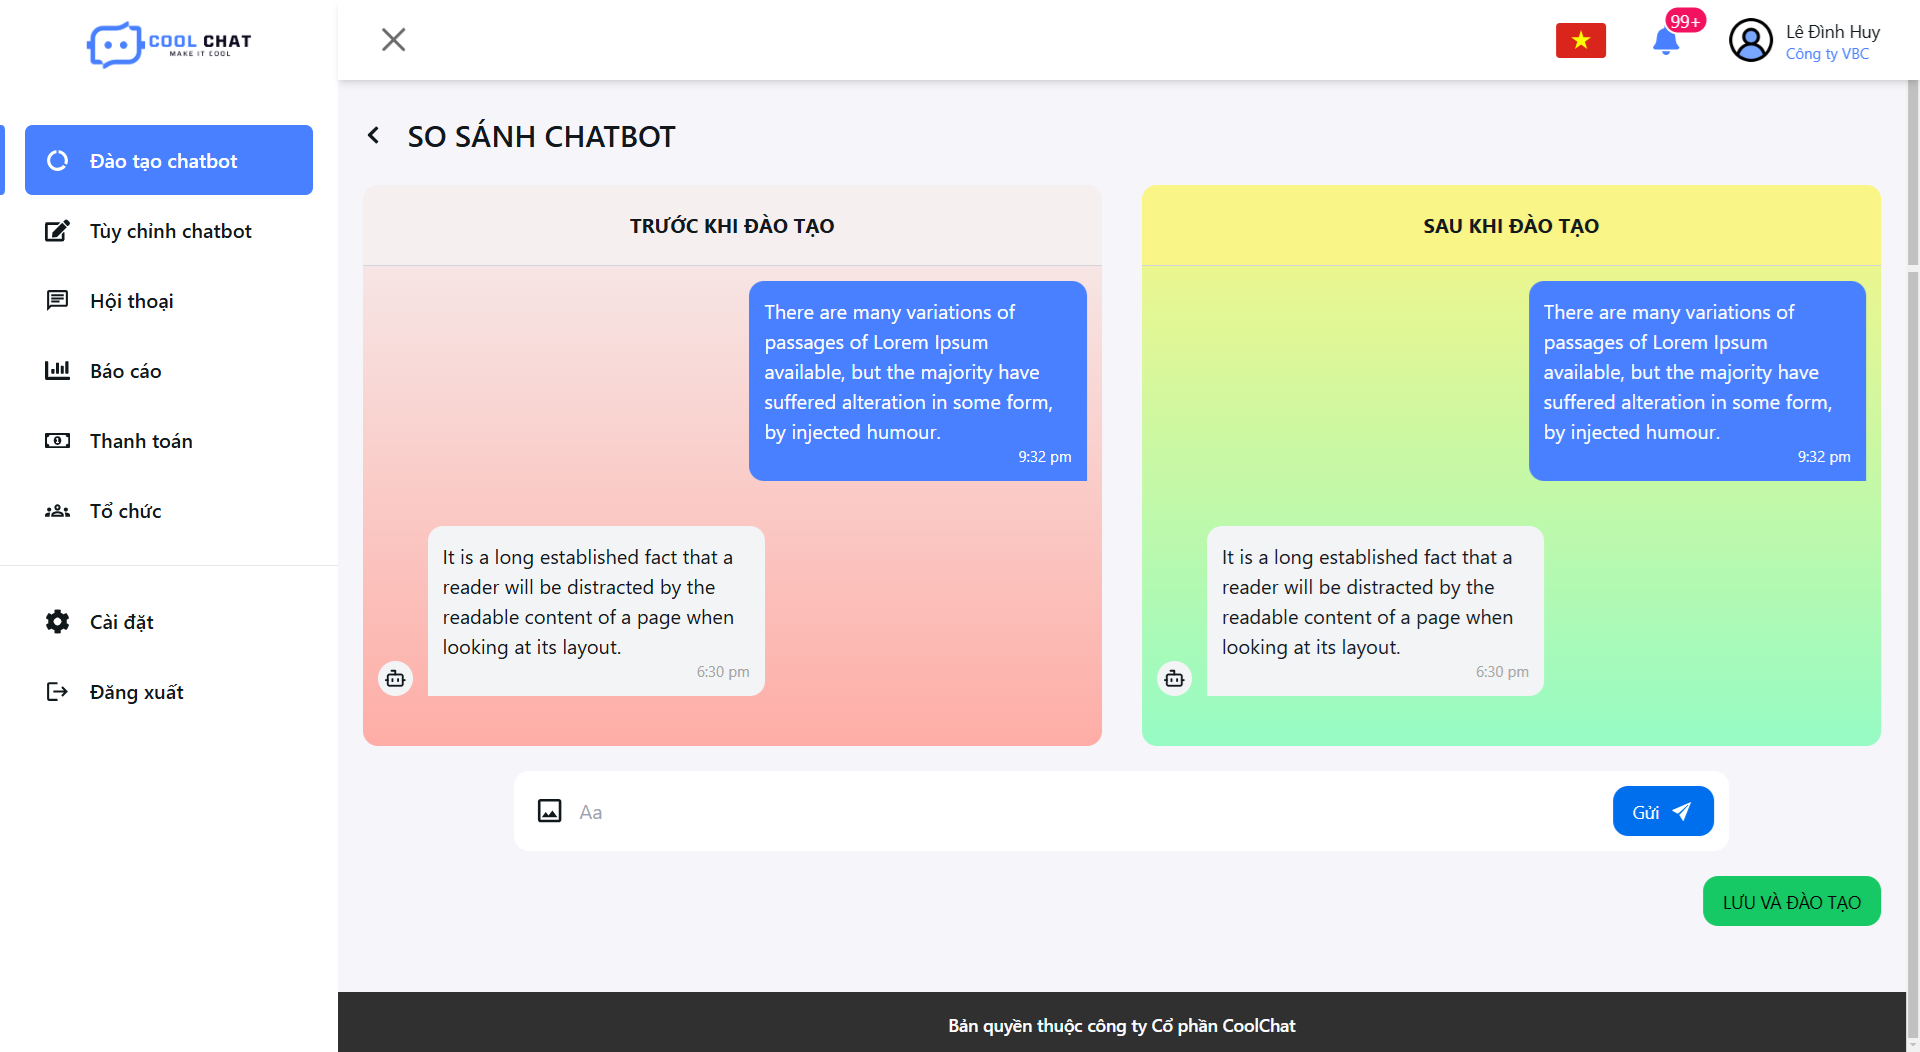
\includegraphics[width=1\textwidth]{Figma/chatbot_comparison_imple.png}}
	\vspace{0.5cm}
	\caption{Giao diện thêm tri thức dạng tập tin}
	\label{fig:enter-label}
\end{figure}
\begin{figure}[H]
	\centering
	\fbox{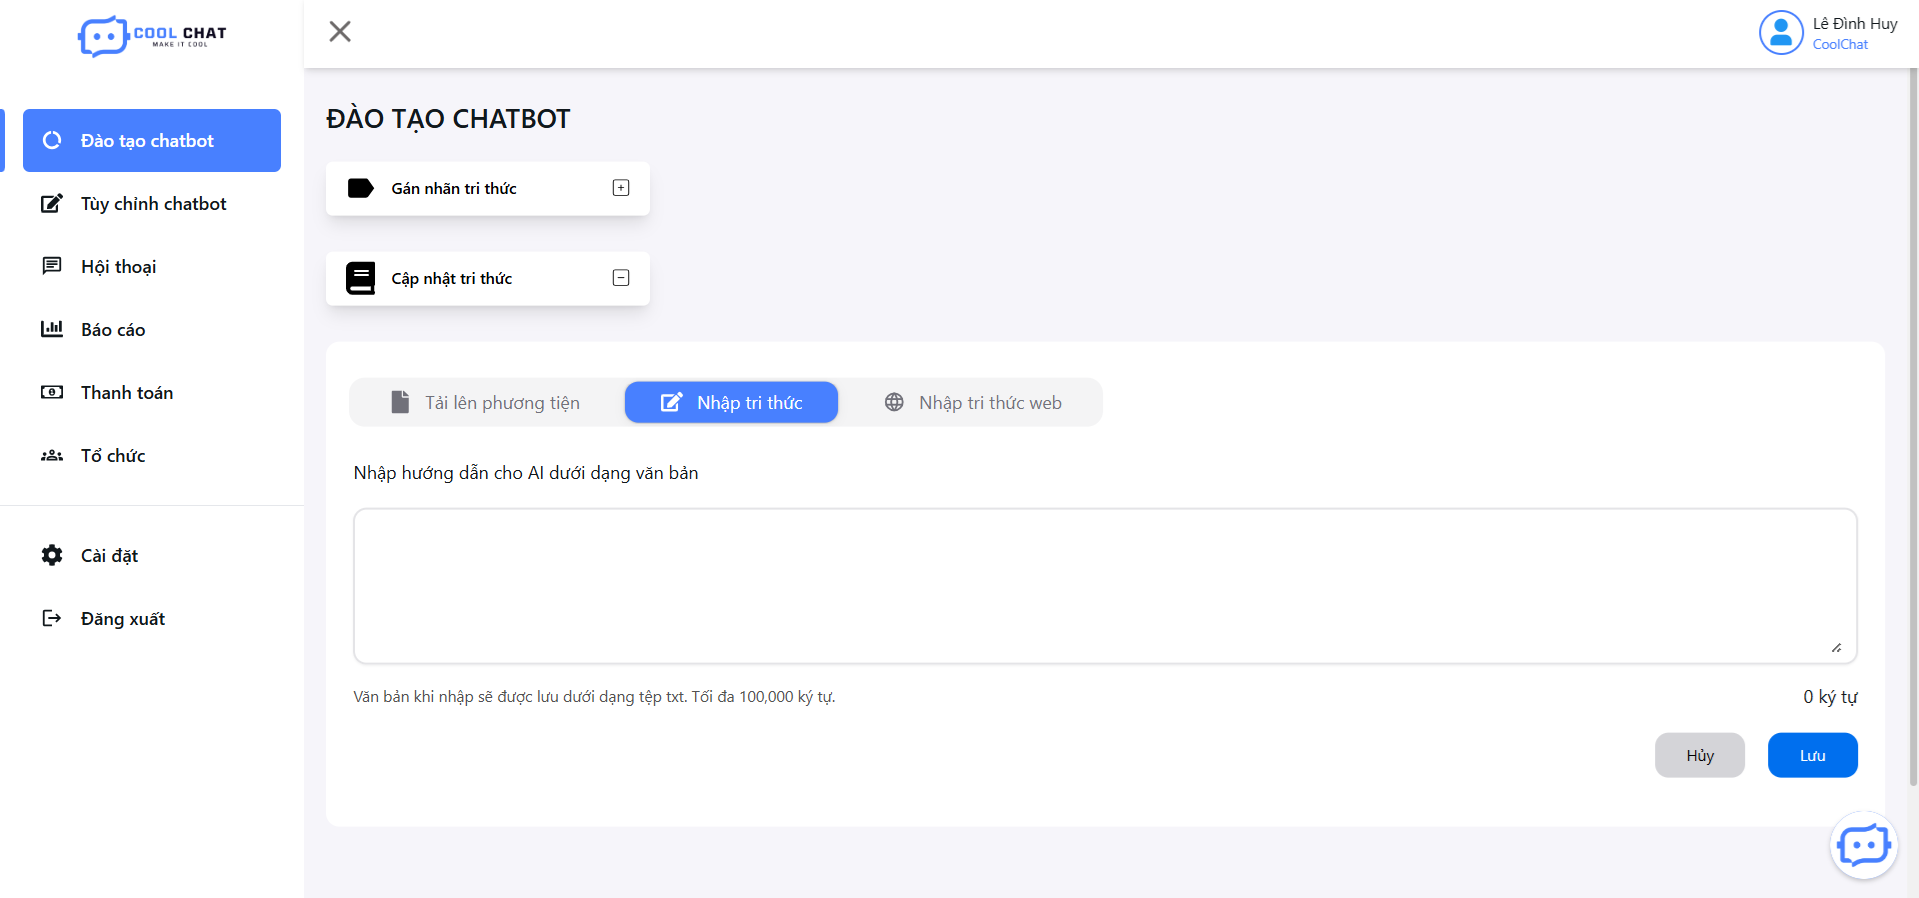
\includegraphics[width=1\textwidth]{Figma/add_text.png}}
	\vspace{0.5cm}
	\caption{Giao diện thêm tri thức dạng văn bản}
	\label{fig:enter-label}
\end{figure}
\begin{figure}[H]
	\centering
	\fbox{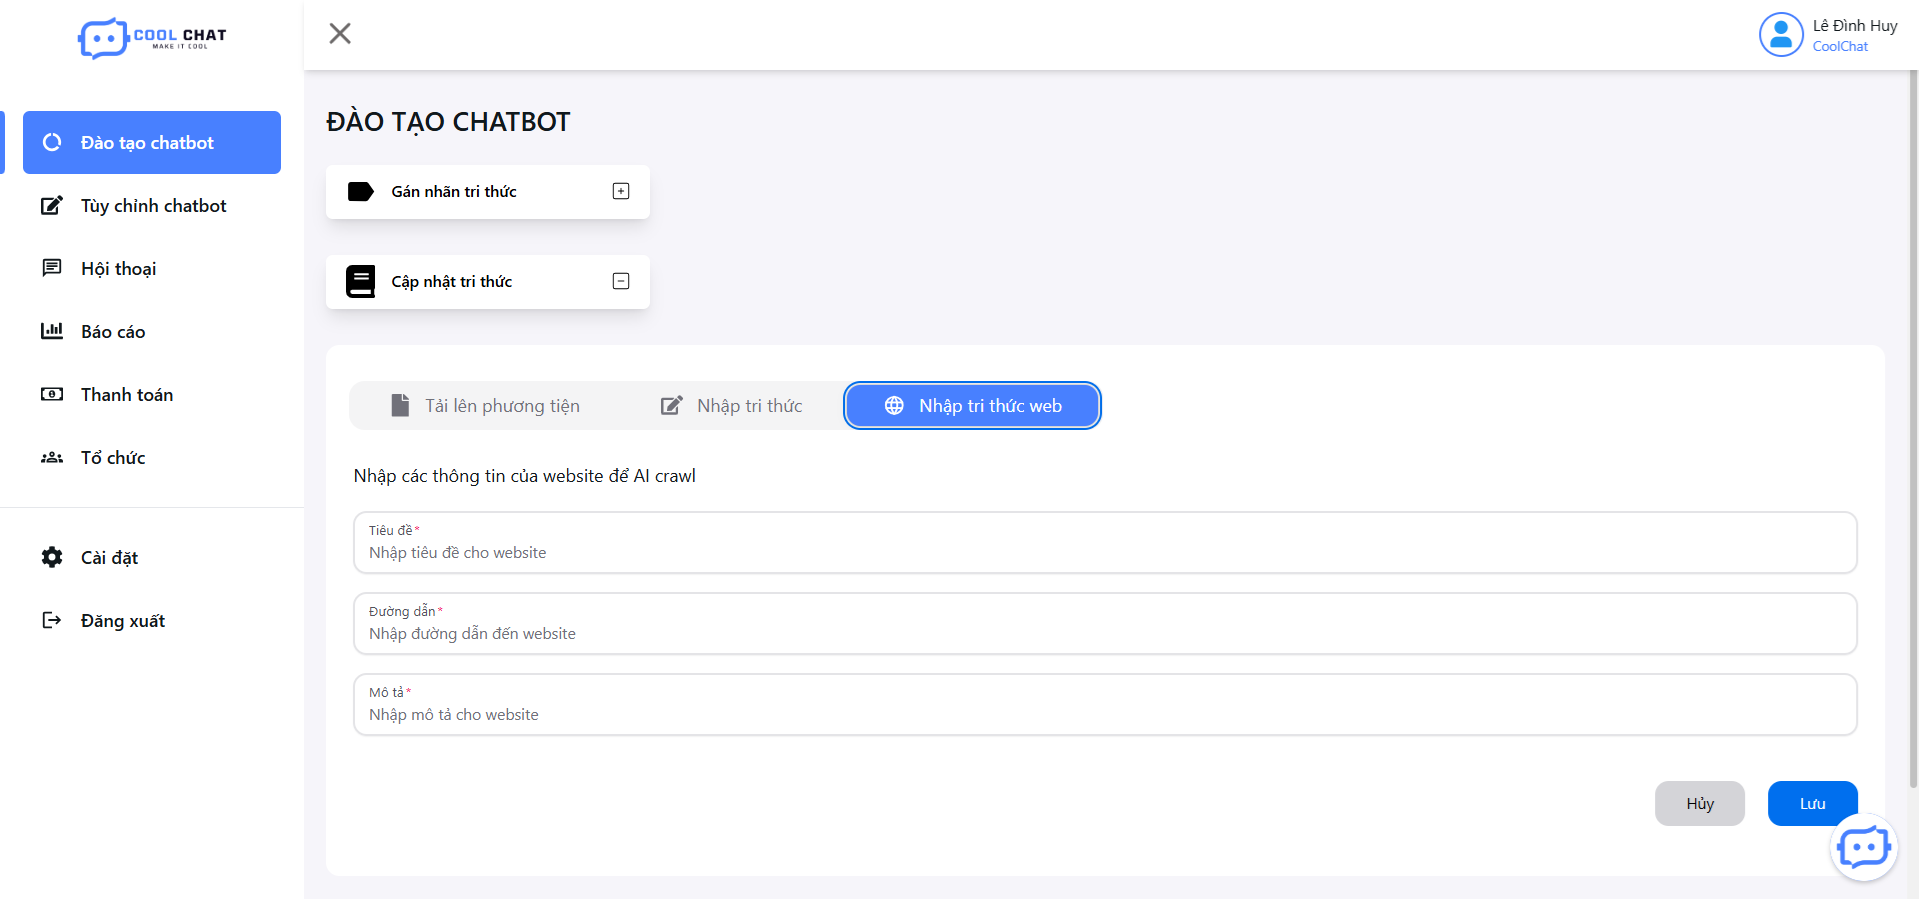
\includegraphics[width=1\textwidth]{Figma/add_web.png}}
	\vspace{0.5cm}
	\caption{Giao diện thêm tri thức dạng website}
	\label{fig:enter-label}
\end{figure}

Ngoài ra, người dùng có thể kiểm tra hoạt động của chatbot của mình trước khi tích hợp bằng hộp chat nằm bên góc phải dưới cùng như hình 81.
\begin{figure}[H]
	\centering
	\fbox{
\includegraphics[width=0.5\textwidth]{Figma/chatbox.png}}
	\vspace{0.5cm}
	\caption{Giao diện hộp chat kiểm thử}
	\label{fig:enter-label}
\end{figure}

Giao diện sẽ chứa đầy đủ các nội dung cần thiết, kể cả các lưu ý cho người dùng.
\subsubsection{Trang Tùy chỉnh chatbot}
Trang Tùy chỉnh chatbot dành cho vai trò Chủ sở hữu hoặc Quản trị viên.

Người dùng có thể cấu hình giao diện chatbot của tổ chức bằng cách chỉnh sửa đa dạng các thông tin, màu sắc, kích thước, ảnh,... như hình 82. Việc người dùng muốn xem giao diện trước khi lưu hoặc khôi phục giao diện mặc định cũng được hệ thống hỗ trợ đầy đủ.
\begin{figure}[H]
	\centering
	\fbox{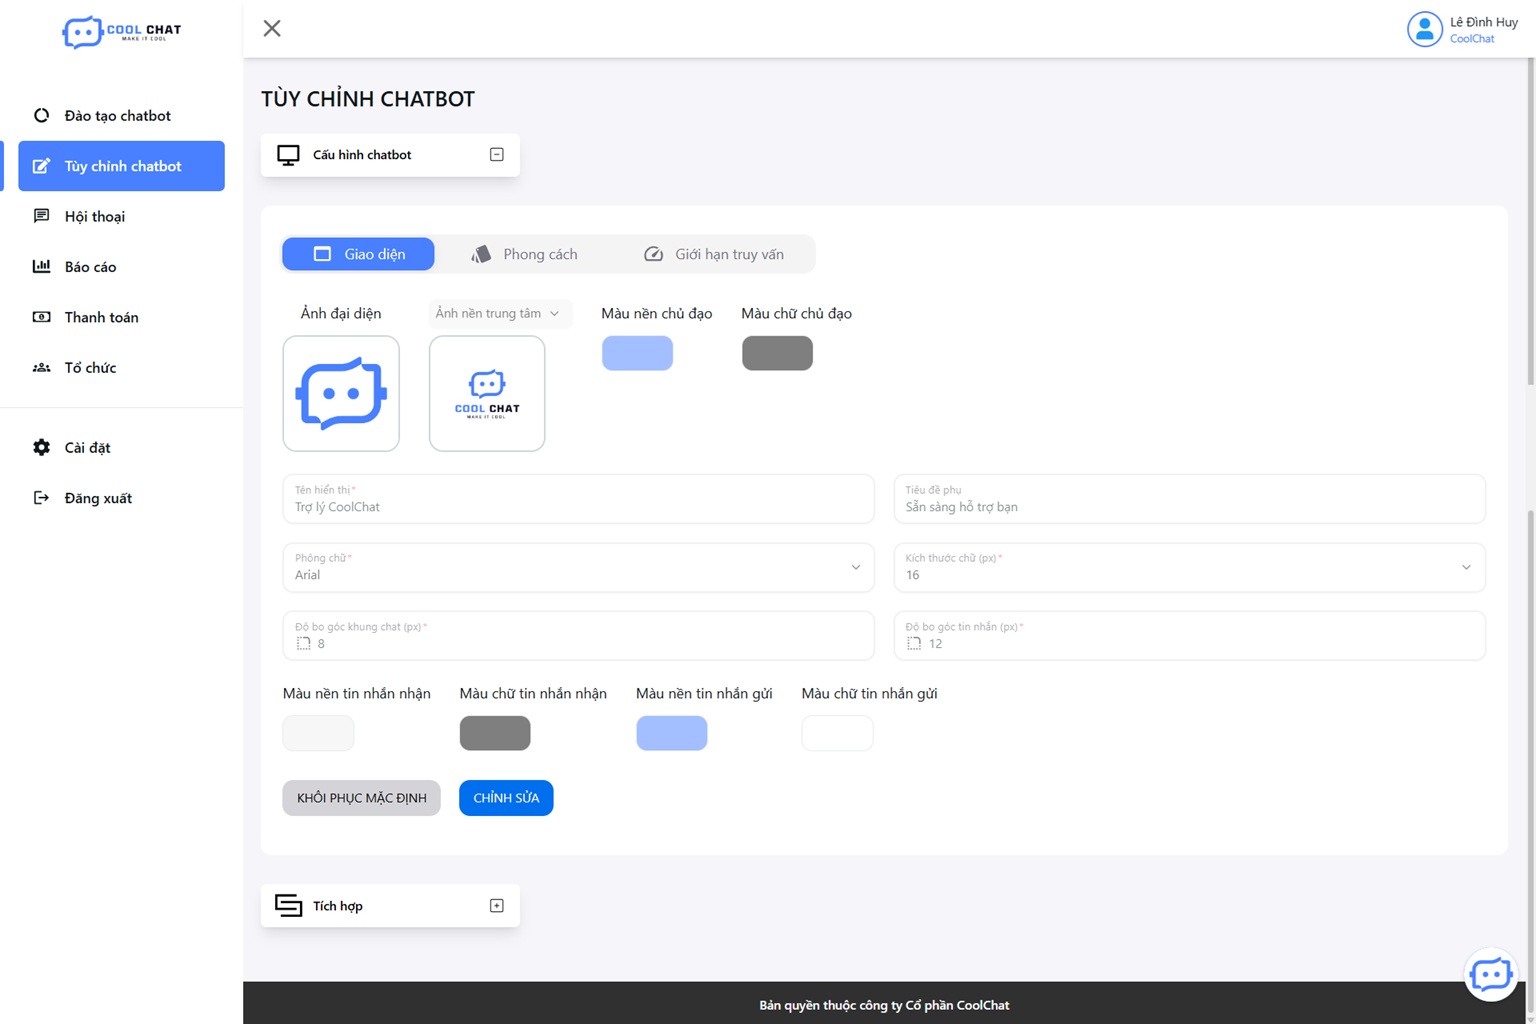
\includegraphics[width=1\textwidth]{Figma/chatboteditting_imple.png}}
	\vspace{0.5cm}
	\caption{Giao diện tùy chỉnh giao diện chatbot}
	\label{fig:enter-label}
\end{figure}

Thêm vào đó, người dùng còn có thể tùy chỉnh phong cách chatbot với tone giọng, các tin nhắn mặc định và cài đặt giới hạn truy vấn như hình 83 và 84, giúp cho chatbot được hoạt động một cách hiệu quả, tránh các trường hợp phá hoại.
\begin{figure}[H]
	\centering
	\fbox{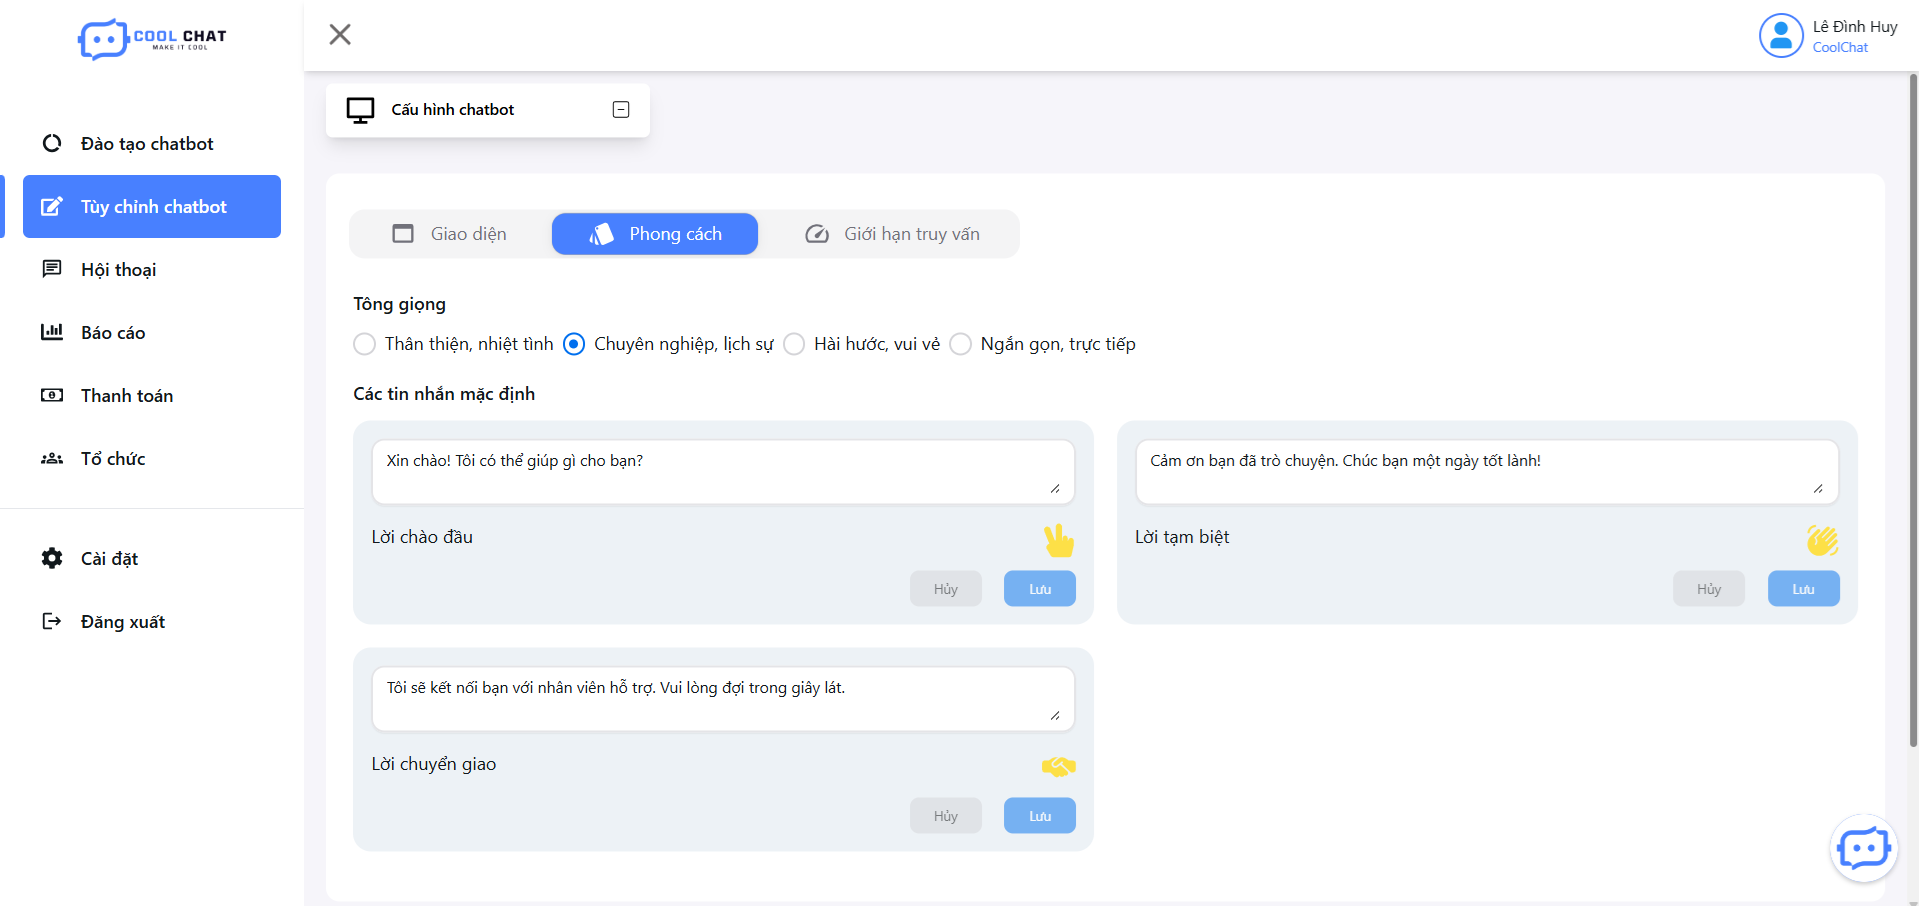
\includegraphics[width=1\textwidth]{Figma/chatbot_edit_imple_2.png}}
	\vspace{0.5cm}
	\caption{Giao diện tùy chỉnh phong cách chatbot}
	\label{fig:enter-label}
\end{figure}
\begin{figure}[H]
	\centering
	\fbox{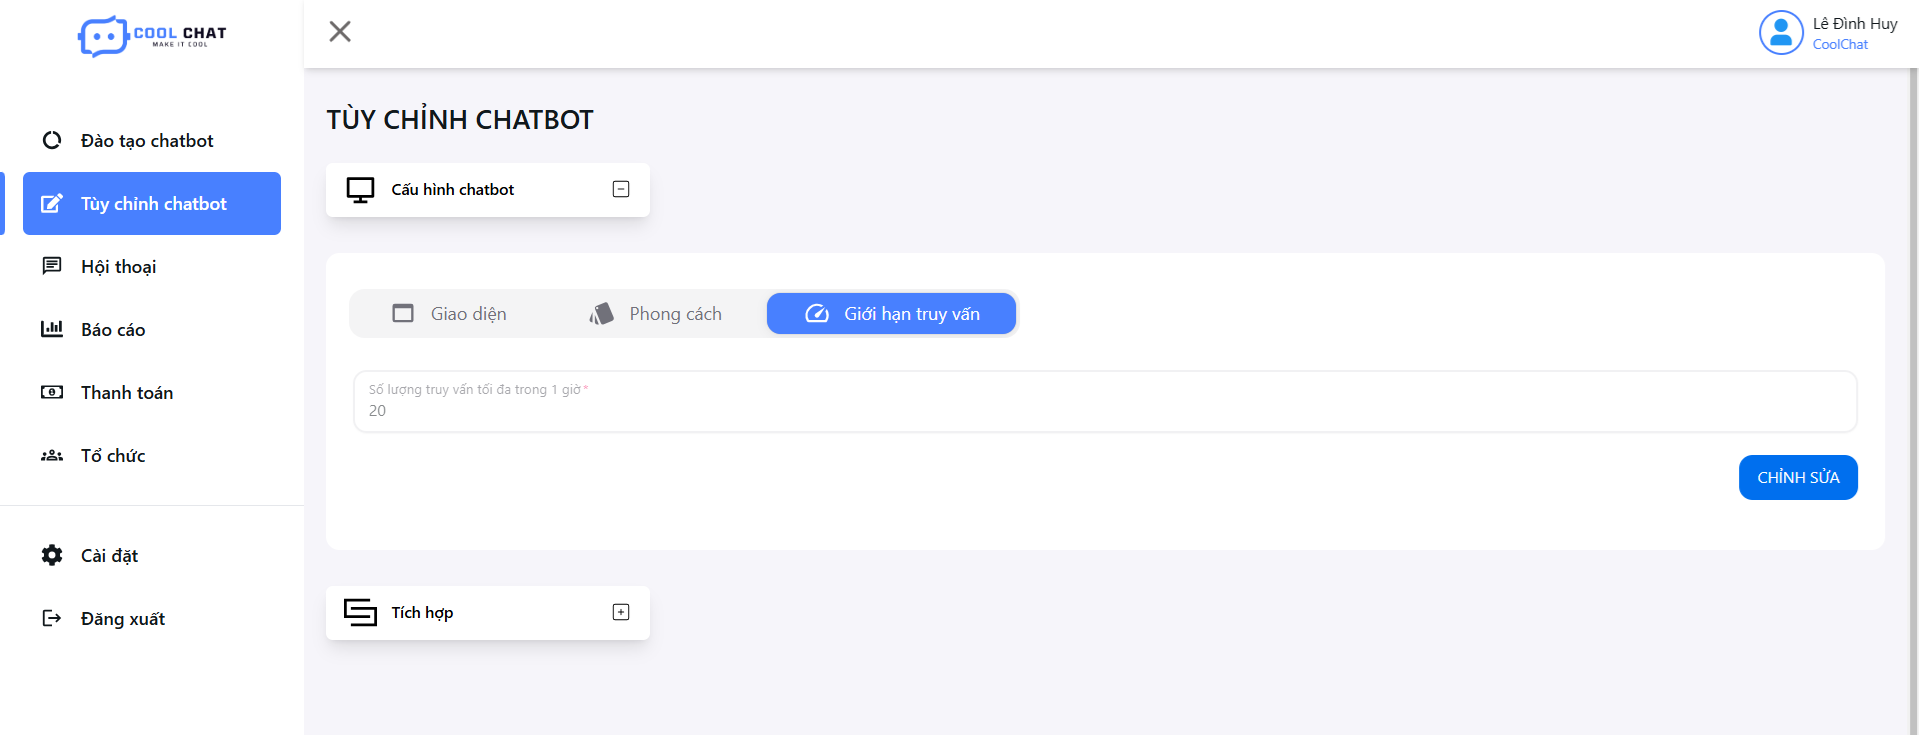
\includegraphics[width=1\textwidth]{Figma/chatbot_edit_imple_3.png}}
	\vspace{0.5cm}
	\caption{Giao diện cài đặt giới hạn truy vấn}
	\label{fig:enter-label}
\end{figure}

Mục Tích hợp sẽ nằm trong trang Tùy chỉnh chatbot được thể hiện ở hình 85. Màn hình sẽ hiển thị đoạn mã nhúng và hướng dẫn. Để giới hạn tích hợp, người dùng có thể quản lý các tên miền cho phép hiển thị.
\begin{figure}[H]
	\centering
	\fbox{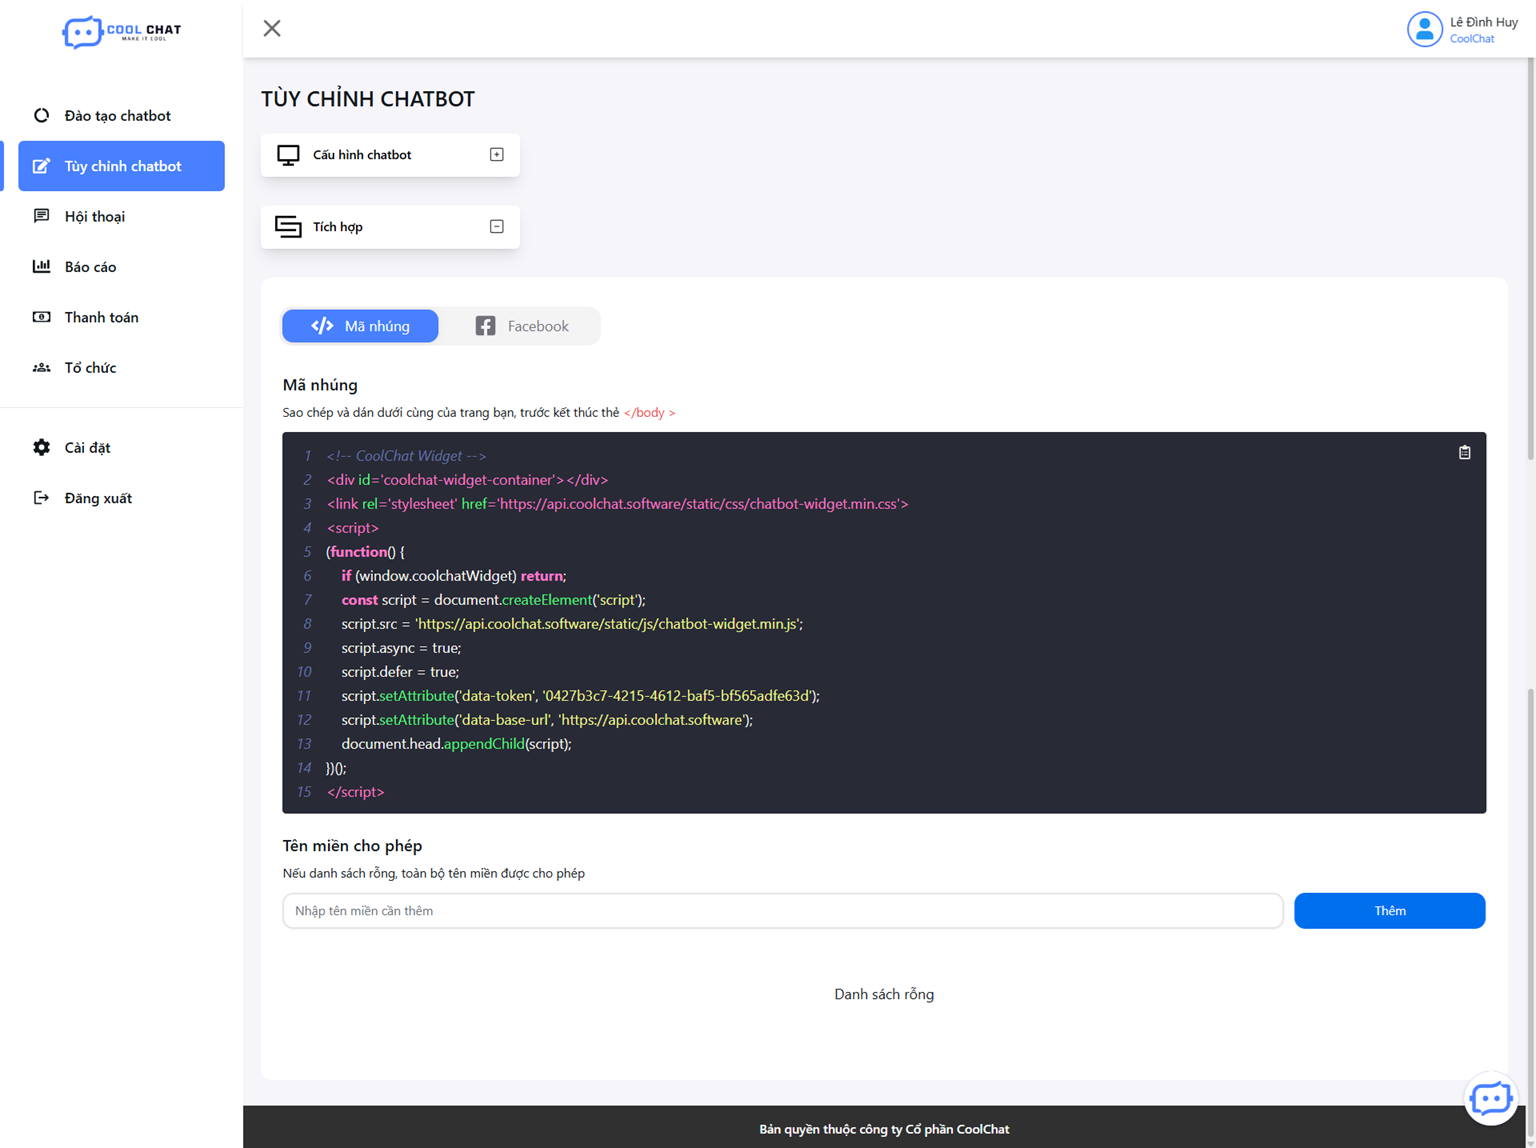
\includegraphics[width=1\textwidth]{Figma/tichhop.png}}
	\vspace{0.5cm}
	\caption{Giao diện tích hợp}
	\label{fig:enter-label}
\end{figure}
\subsubsection{Trang Hội thoại}
Chức năng hội thoại sẽ dành cho cả 3 role, nhưng sẽ khác nhau giữa Chủ sở hữu và Quản trị viên với Nhân viên CSKH.

Màn hình hội thoại như hình 86 sẽ chứa tất cả cuộc hội thoại của tổ chức dành cho Chủ sở hữu và Quản trị viên, còn Nhân viên chỉ được xem những đoạn hội thoại được giao cho mình. Người dùng có thể tìm kiếm và lọc để tìm kiếm hội thoại một cách nhanh nhất.
\begin{figure}[H]
	\centering
	\fbox{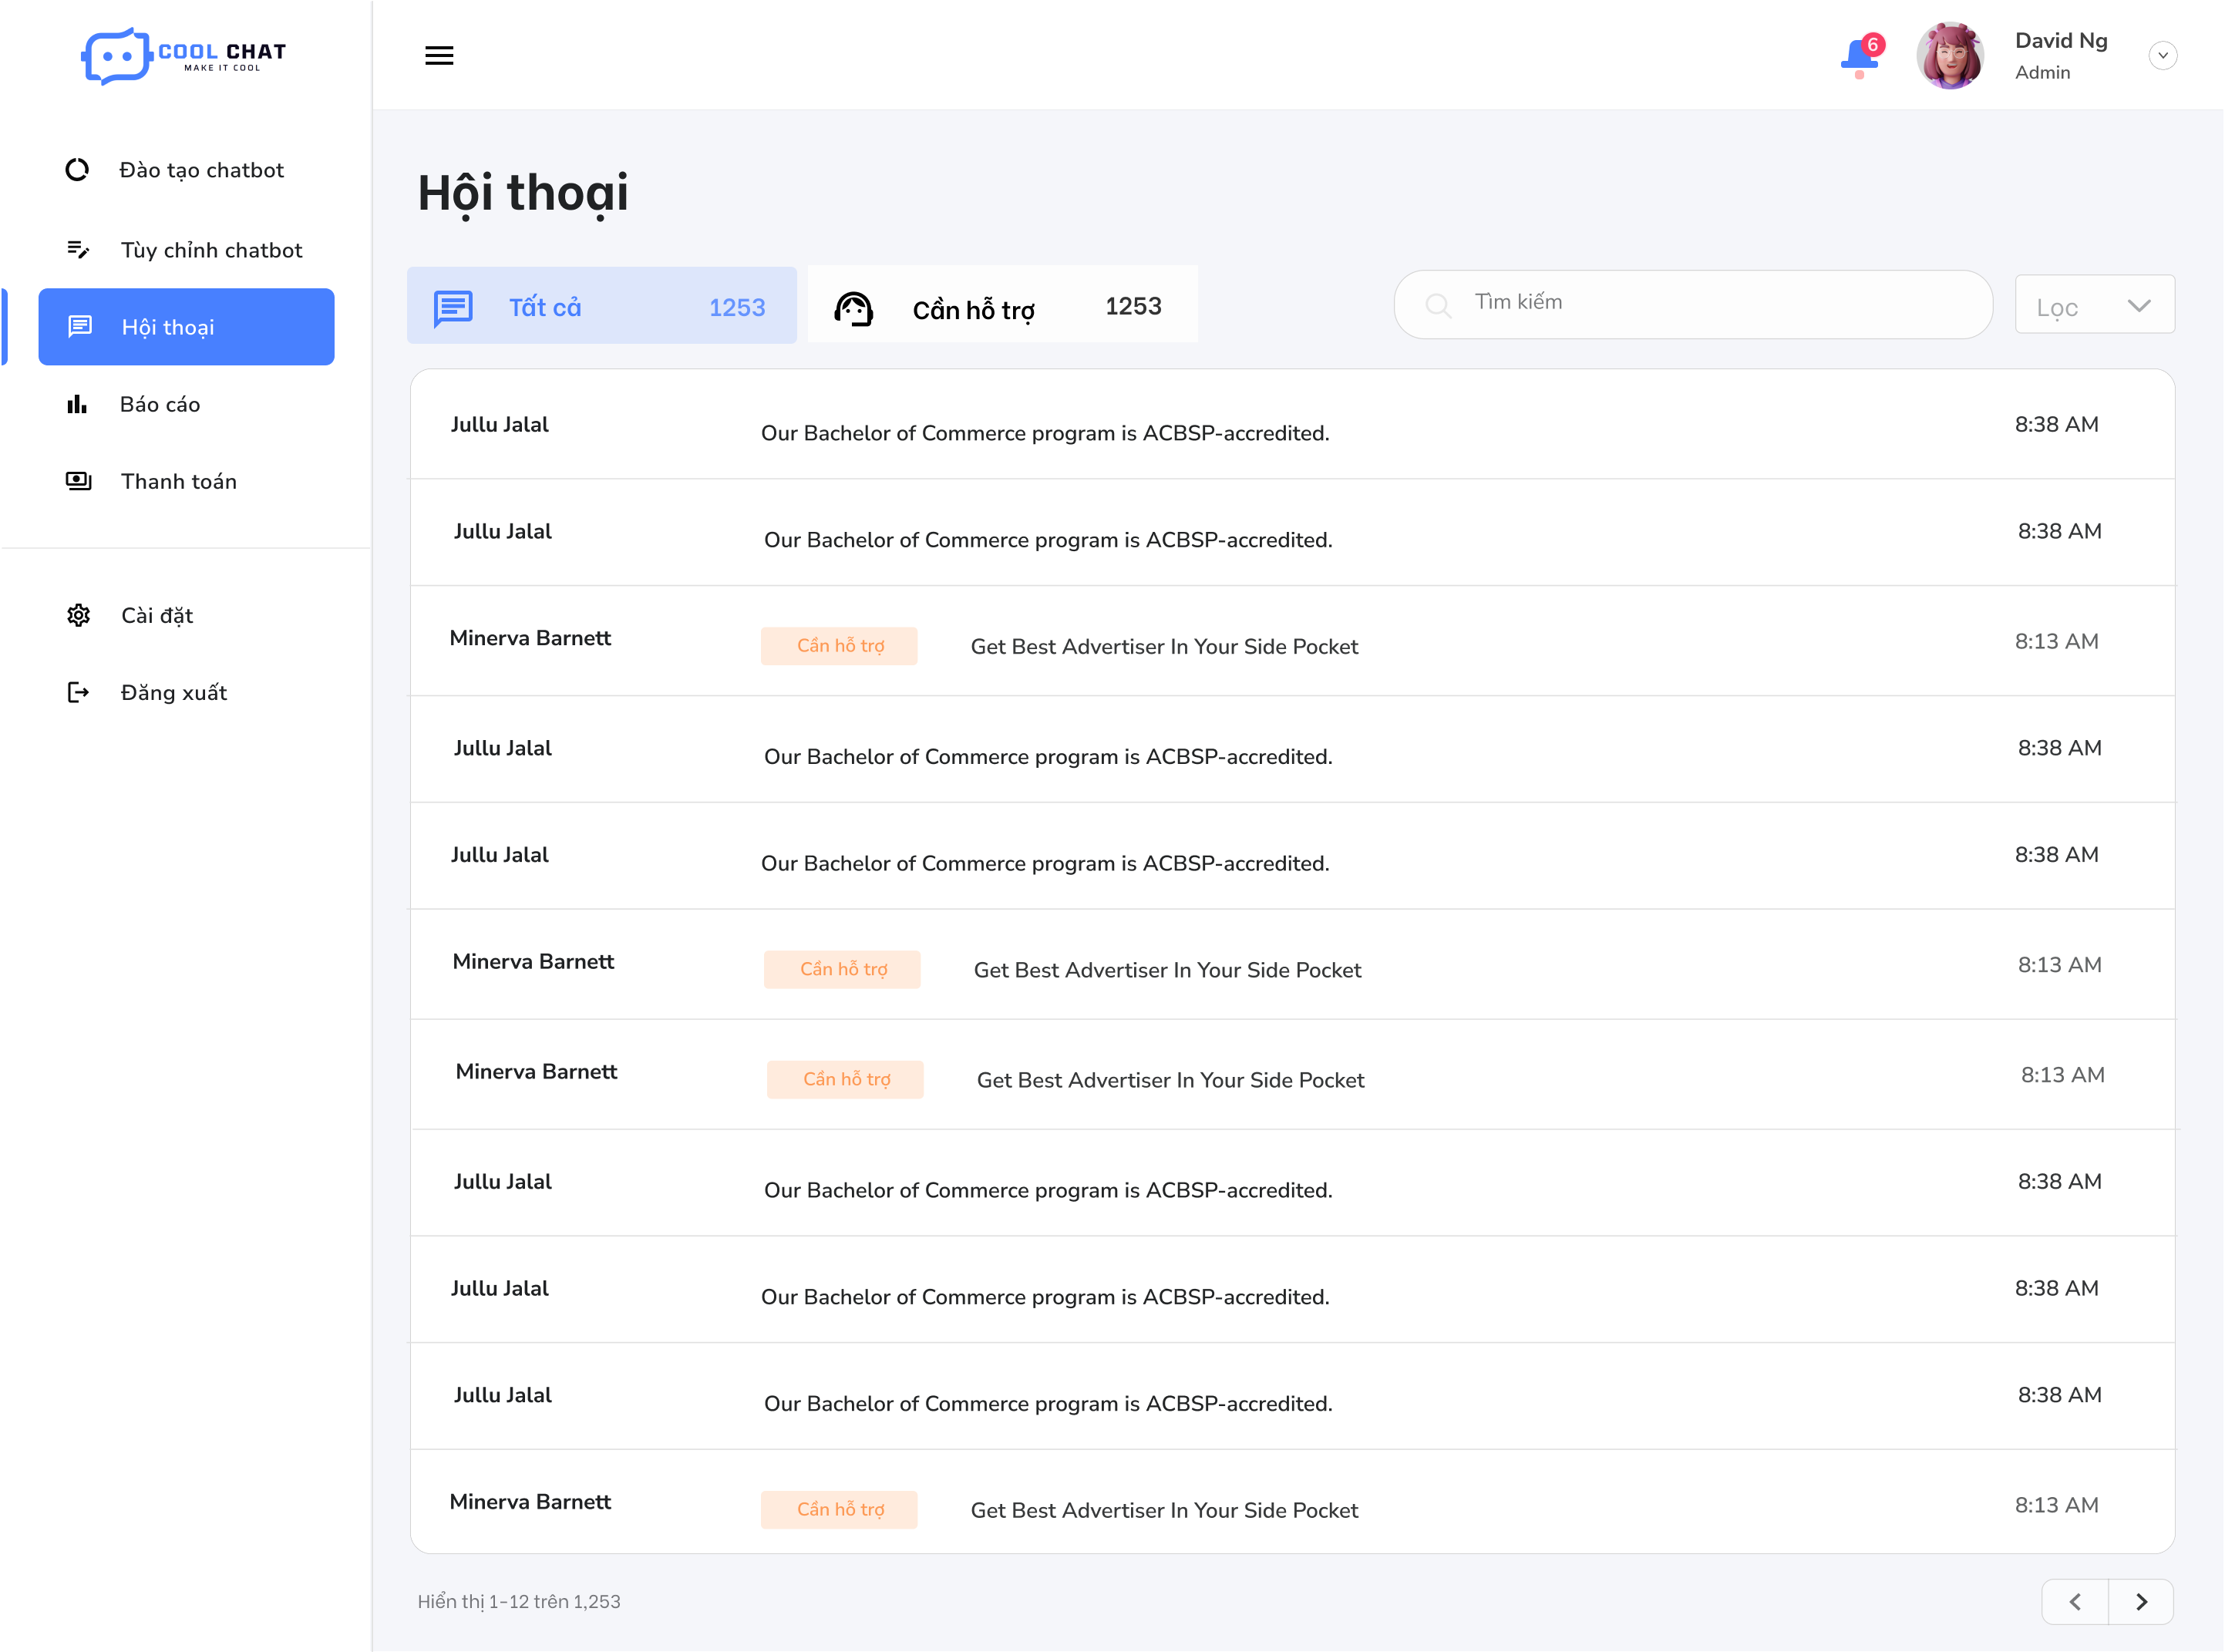
\includegraphics[width=1\textwidth]{Figma/chat_1.png}}
	\vspace{0.5cm}
	\caption{Giao diện hội thoại}
	\label{fig:enter-label}
\end{figure}

Khi chuyển sang tab Cần hỗ trợ như hình 87, màn hình sẽ lọc ra những hội thoại cần hỗ trợ để hỗ trợ khách hàng một cách nhanh nhất.
\begin{figure}[H]
	\centering
	\fbox{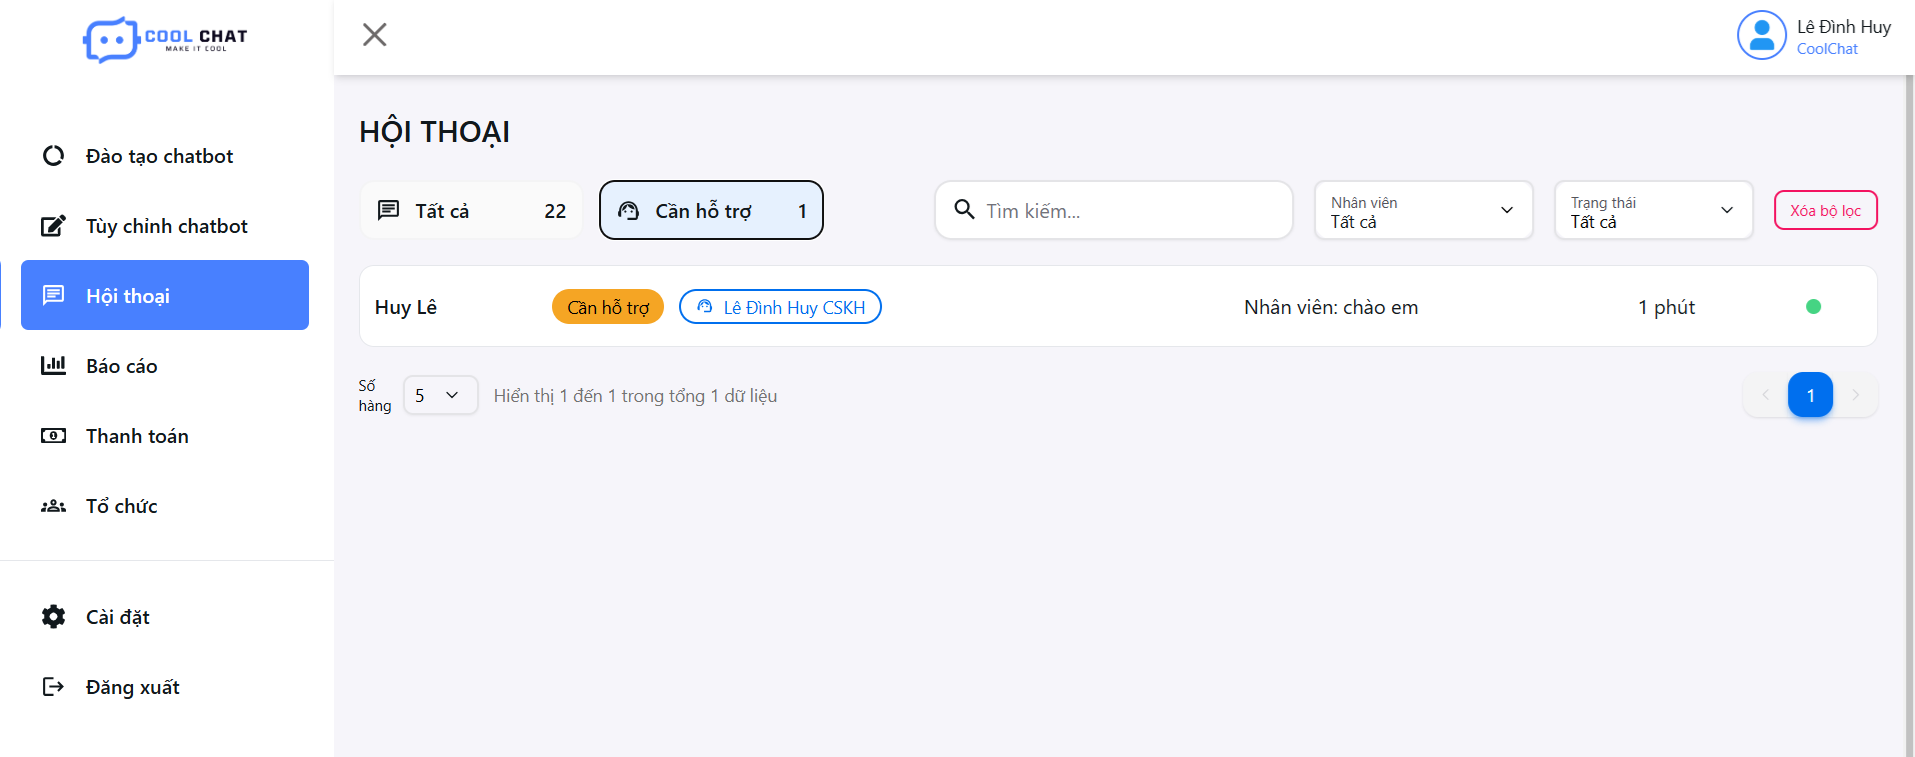
\includegraphics[width=1\textwidth]{Figma/chat_2.png}}
	\vspace{0.5cm}
	\caption{Giao diện hội thoại cần hỗ trợ}
	\label{fig:enter-label}
\end{figure}

Màn hình xem chi tiết hội thoại cũng tương ứng với từng vai trò với các chức năng cho phép như hình 88. Màn hình sẽ hiển thị tên khách hàng, trạng thái, tên nhân viên (nếu có), tất cả lịch sử tin nhắn của hệ thống, chatbot và nhân viên. Tin nhắn của bản thân sẽ màu xanh, còn không phải sẽ màu xám. Bên cạnh đó sẽ là thanh thông tin bên phải có thể đóng mở chứa các thông tin chi tiết.

Chủ sở hữu và quản trị viên có thể chuyển hội thoại thành tự động, gán nhân viên và đóng cuộc hội thoại. 

\begin{figure}[H]
	\centering
	\fbox{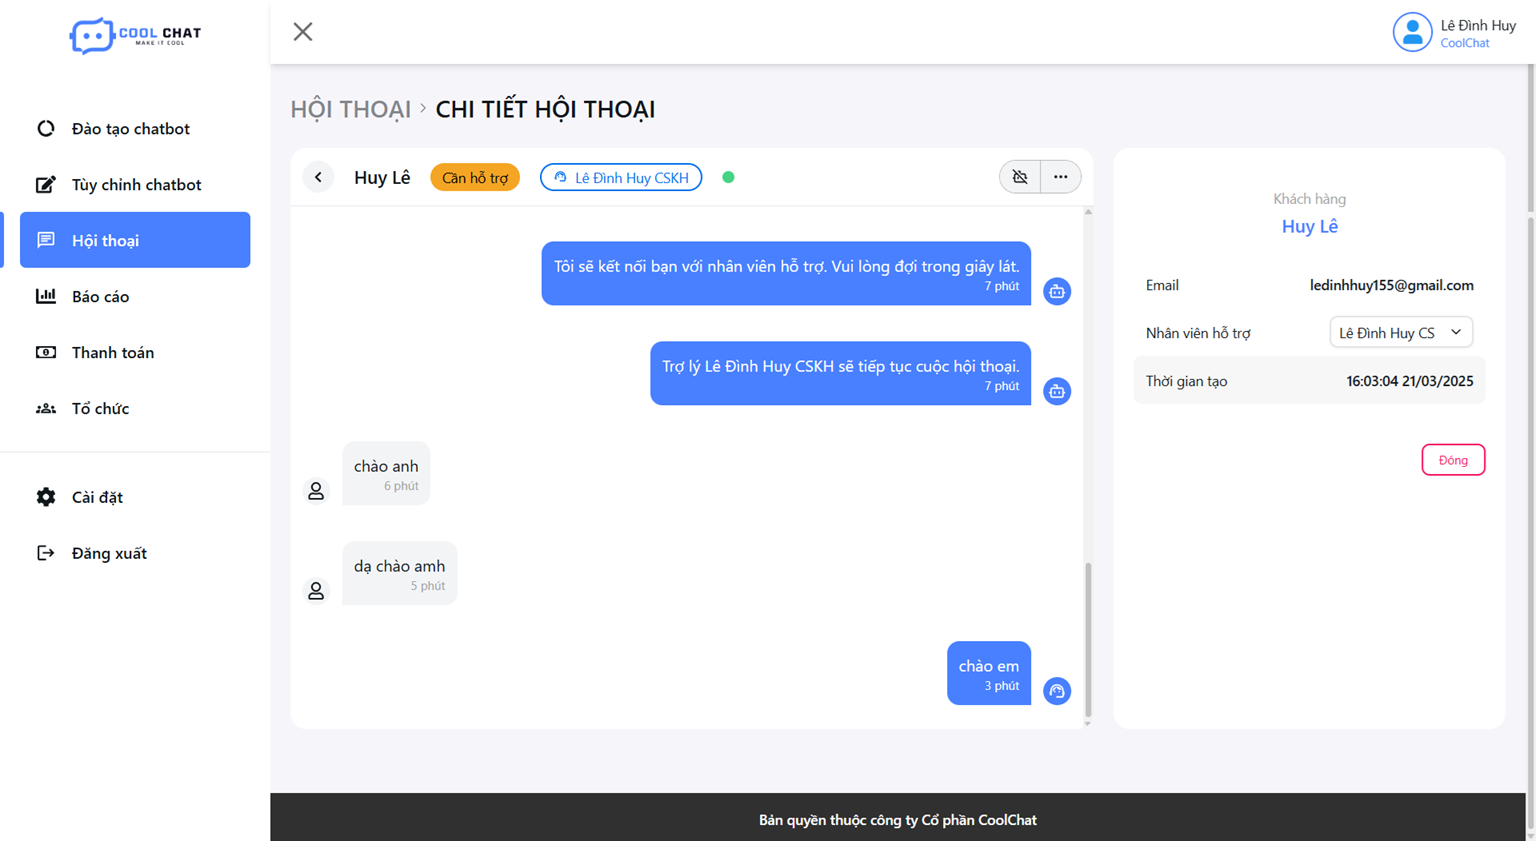
\includegraphics[width=1\textwidth]{Figma/chat_detail_imple.png}}
	\vspace{0.5cm}
	\caption{Giao diện chi tiết hội thoại cho chủ sở hữu và quản trị viên}
	\label{fig:enter-label}
\end{figure}

Nhân viên có thể nhắn tin với khách hàng cần hỗ trợ, chuyển hội thoại thành tự động và đóng cuộc hội thoại như hình 89.
\begin{figure}[H]
	\centering
	\fbox{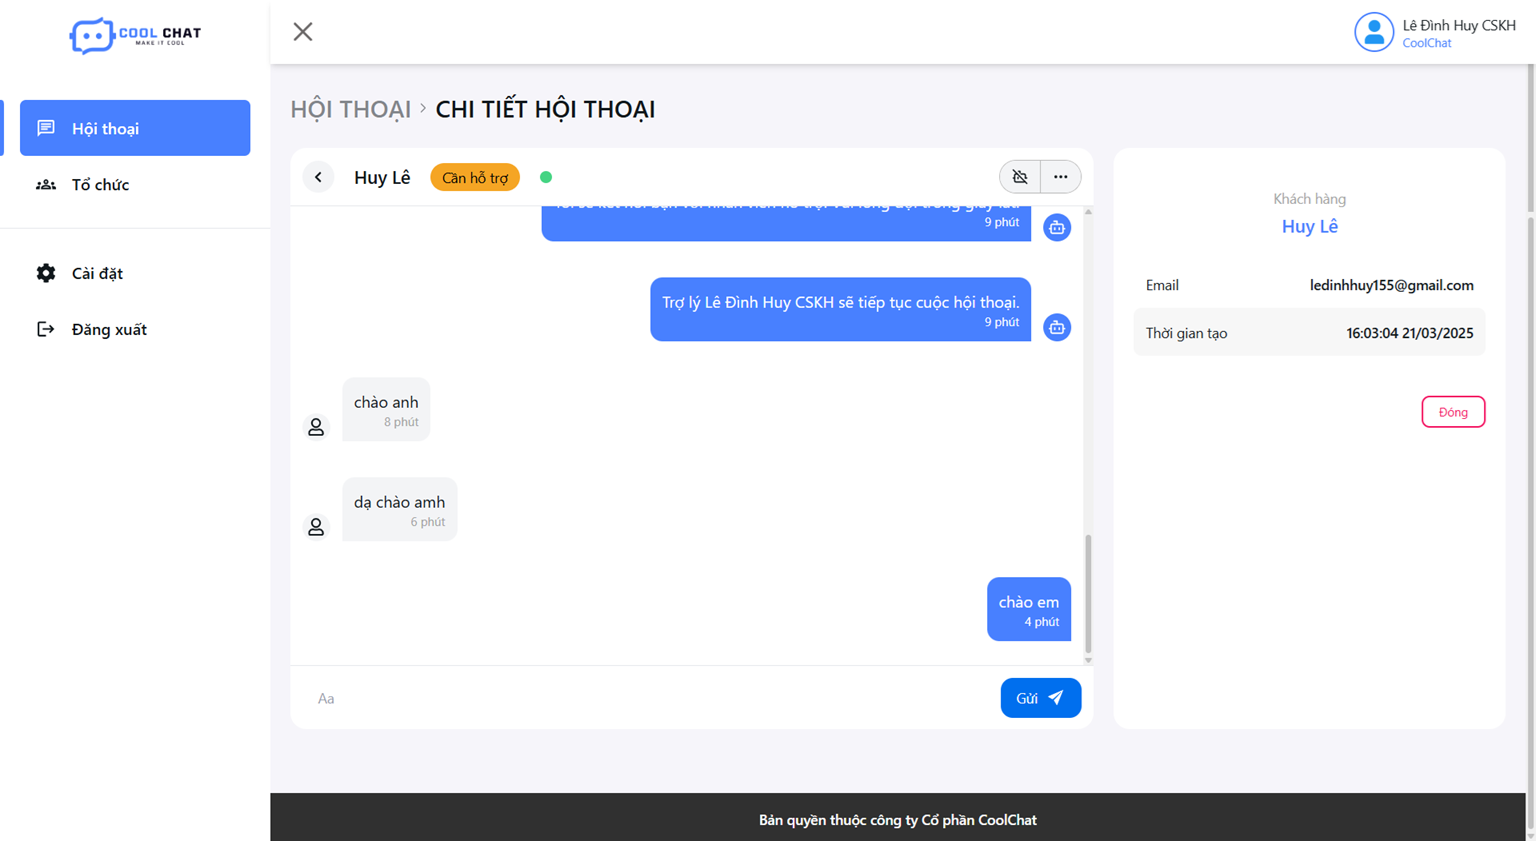
\includegraphics[width=1\textwidth]{Figma/chat_detail_imple_1.png}}
	\vspace{0.5cm}
	\caption{Giao diện chi tiết hội thoại cho chủ sở hữu và quản trị viên}
	\label{fig:enter-label}
\end{figure}
\subsubsection{Trang Báo cáo}
Giao diện trang Báo cáo dành cho Chủ sở hữu và Quản trị viên chỉ đơn giản là hiện thị các số liệu hoạt động của chatbot như số cuộc hội thoại, số yêu cầu hỗ trợ, số tin nhắn và thời lượng các cuộc hội thoại trung bình Bên dưới sẽ là các biểu đồ nhằm cung cấp cho người dùng cái nhìn khách quan về quá trình sử dụng hệ thống và hoạt động của chatbot để có thể đánh giá và đưa ra các quyết định phù hợp. Giao diện được thể hiện trong hình 90.
\begin{figure}[H]
	\centering
	\fbox{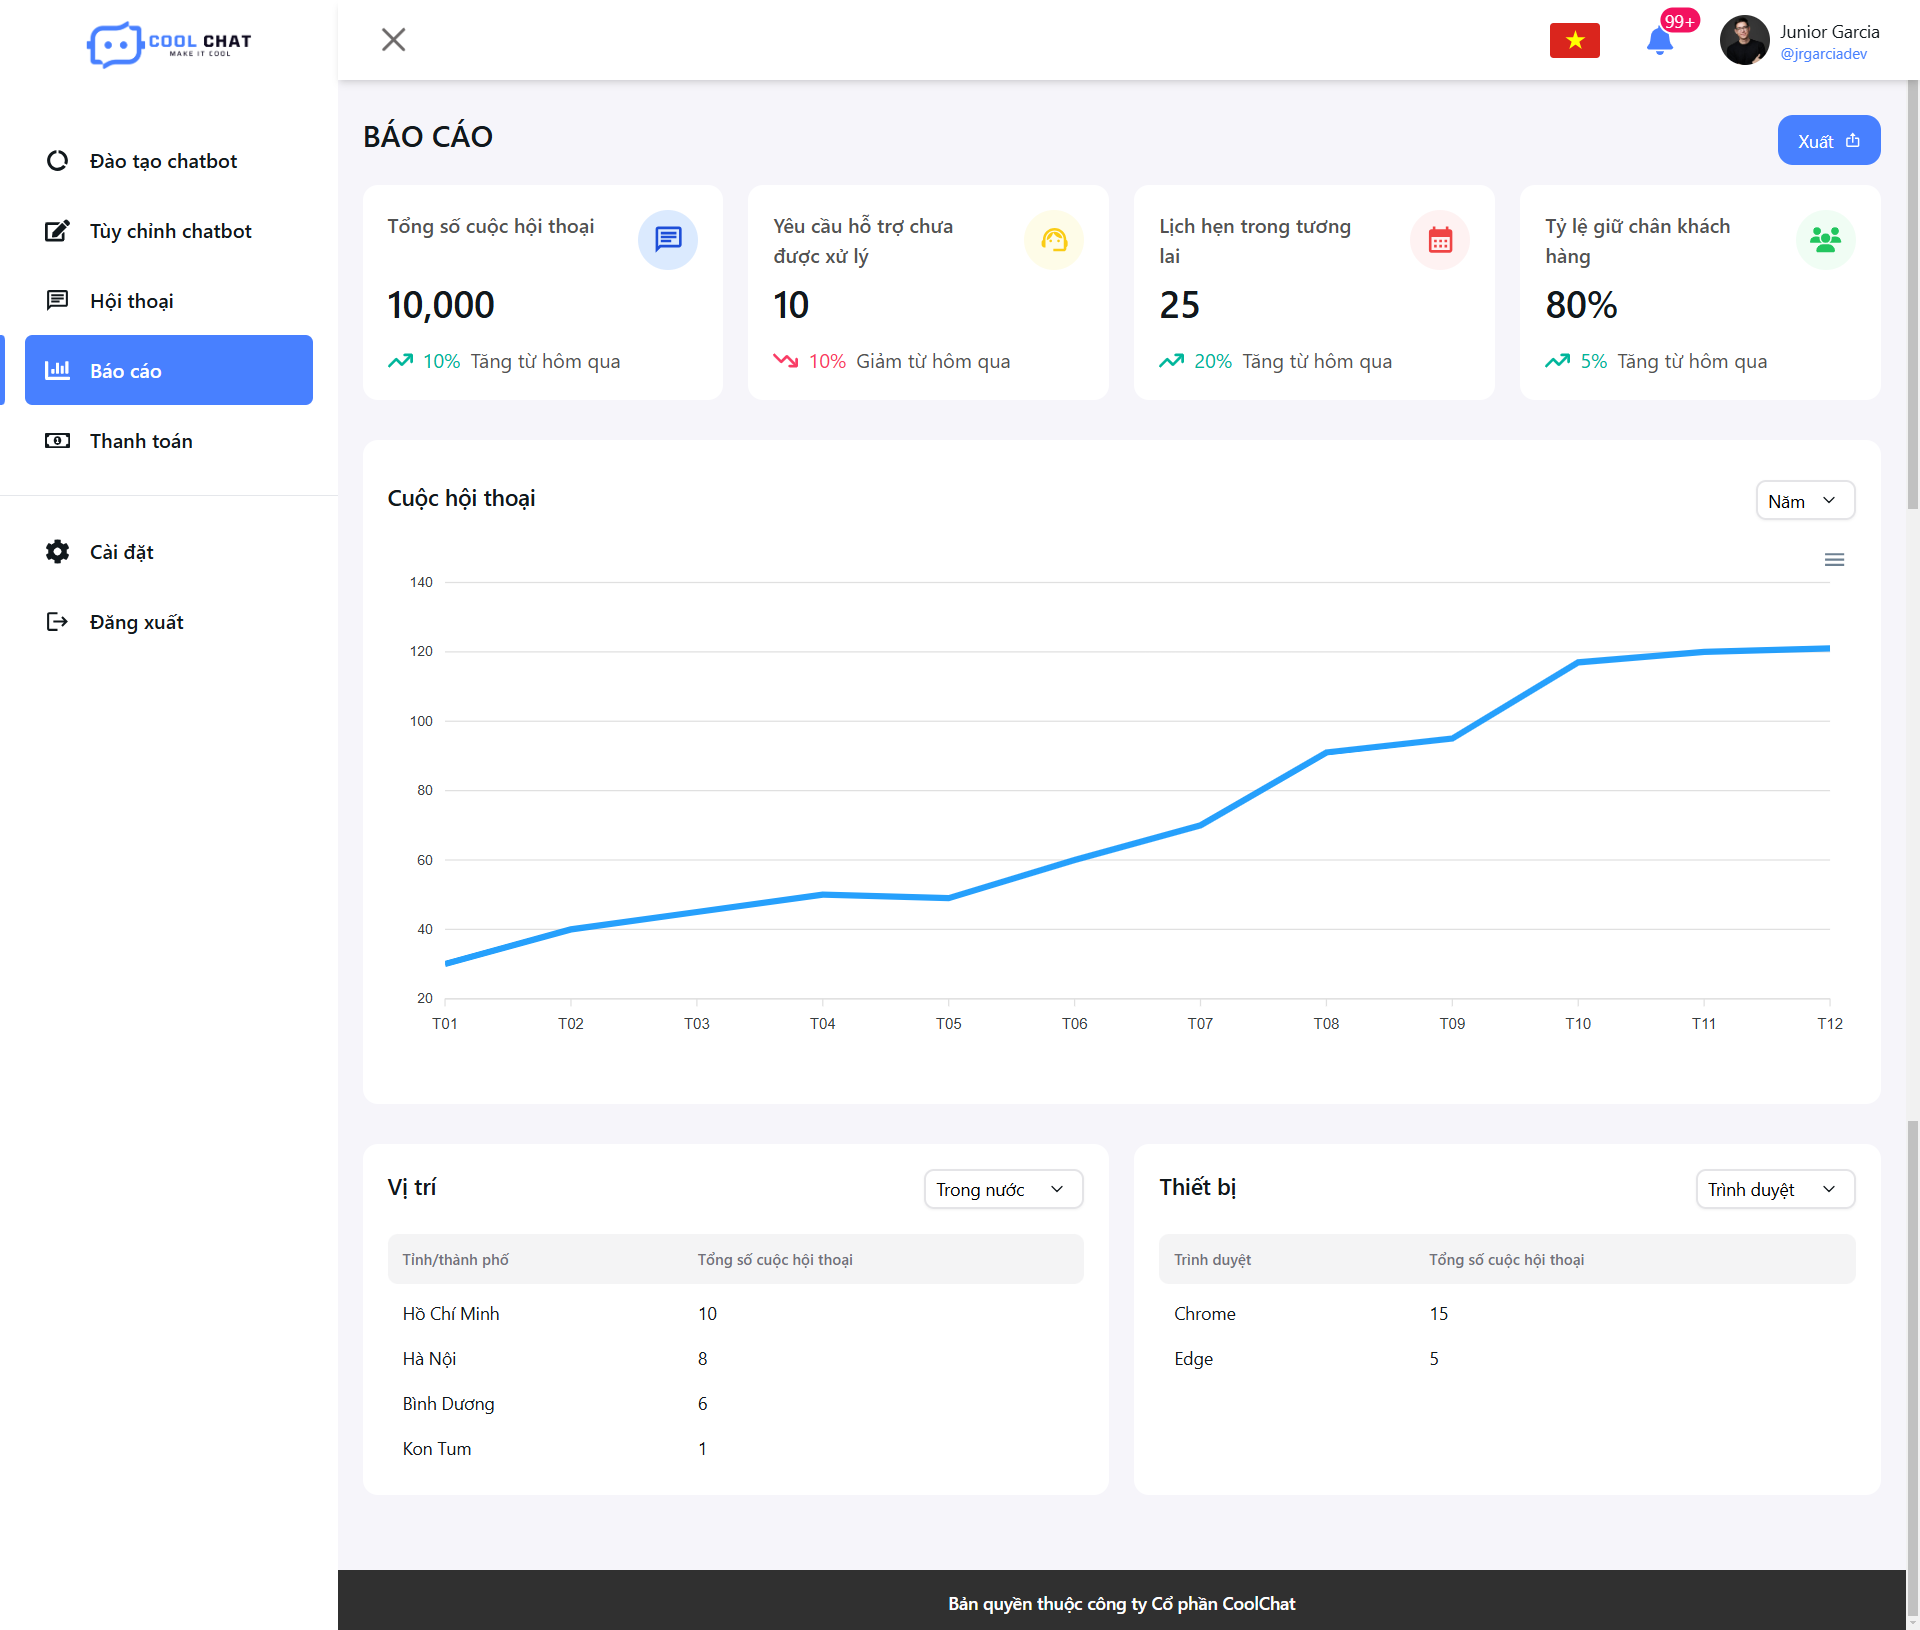
\includegraphics[width=1\textwidth]{Figma/report_imple.png}}
	\vspace{0.5cm}
	\caption{Giao diện báo cáo}
	\label{fig:enter-label}
\end{figure}

Ngoài ra, người dùng có thể lọc theo thời gian hoặc đổi thông tin khác cần hiển thị với các biểu đồ về hội thoại và thanh toán. Việc xuất biểu đồ là cho phép với cả 3 loại biểu đồ, người dùng có thể tùy chọn xuất svg, png hoặc csv như hình 91.
\begin{figure}[H]
	\centering
	\fbox{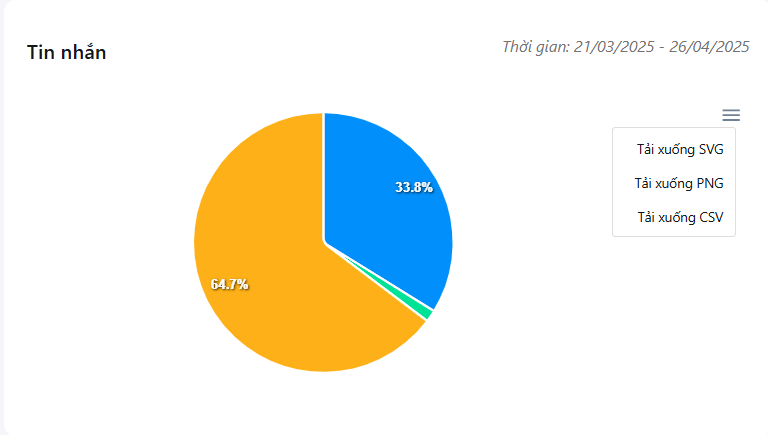
\includegraphics[width=0.5\textwidth]{Figma/export_imple.png}}
	\vspace{0.5cm}
	\caption{Giao diện xuất báo cáo}
	\label{fig:enter-label}
\end{figure}
\subsubsection{Trang Thanh toán}
Trang Thanh toán dành cho Chủ sở hữu và Quản trị viên sẽ hiển thị thông tin của gói đăng ký hiện tại bao gồm tên gói, các mức độ sử dụng của truy vấn AI, kho lưu trữ tài liệu, tài khoản nhân viên và trạng thái gói (nếu còn hạn thì để hạn sử dụng, nếu hết hạn thì để đã hết hạn) như hình 92. Ngoài ra còn có nút gia hạn để người dùng có thể gia hạn thêm thời gian cho gói hiện tại.
\begin{figure}[H]
	\centering
	\fbox{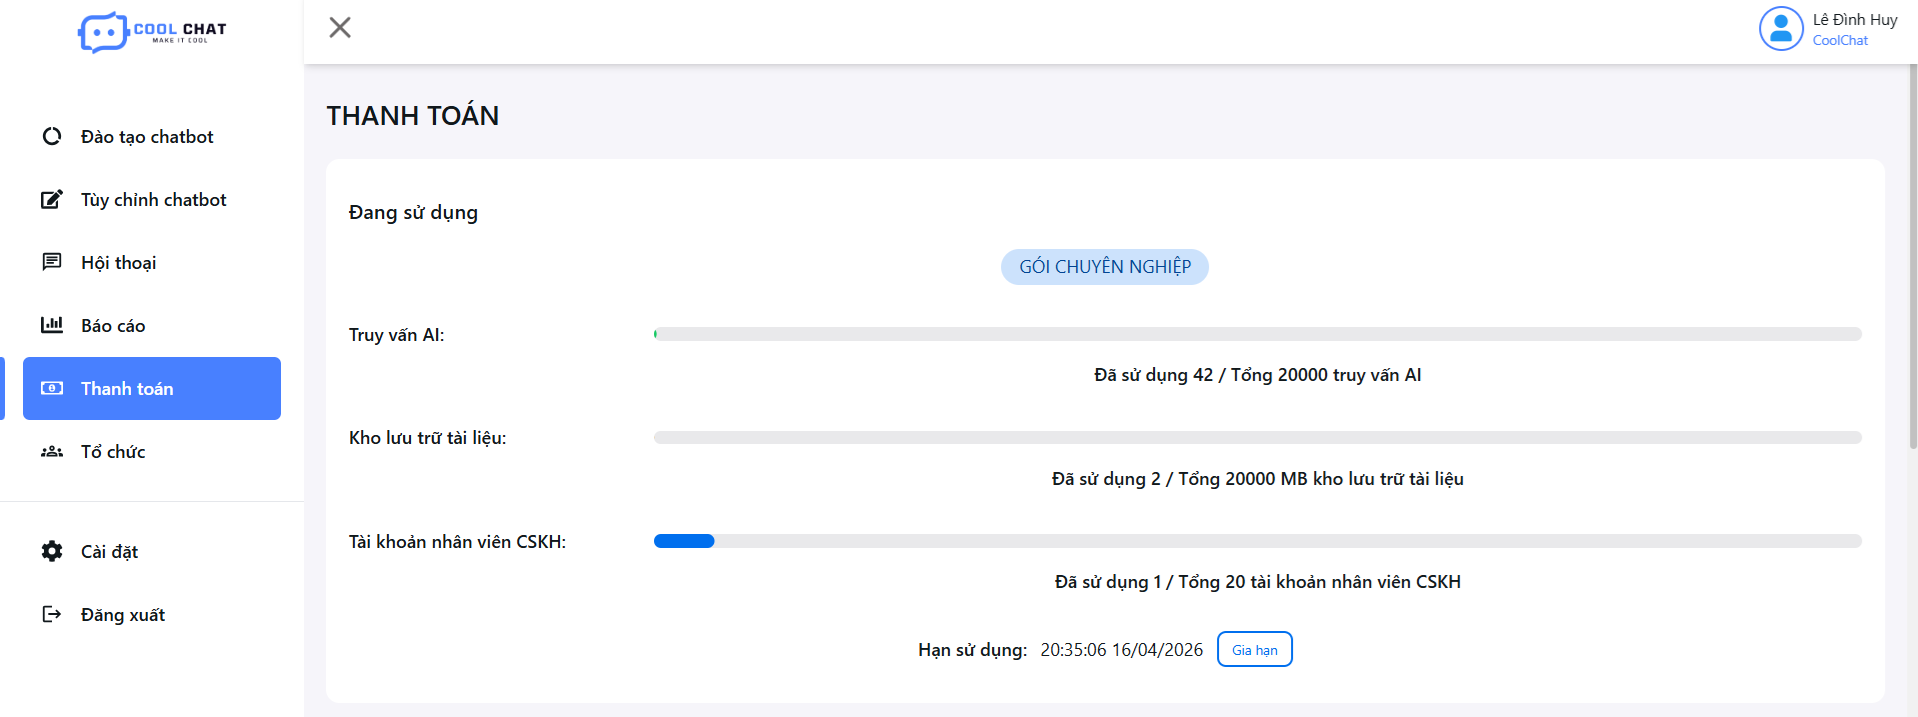
\includegraphics[width=1\textwidth]{Figma/sub_imple1.png}}
	\vspace{0.5cm}
	\caption{Giao diện thông tin gói đăng ký hiện tại}
	\label{fig:enter-label}
\end{figure}

Bên dưới sẽ là thông tin của các gói đăng ký và bổ sung như hình 93 và 94. Người dùng có thể chọn mua và thanh toán nếu được phép.
\begin{figure}[H]
	\centering
	\fbox{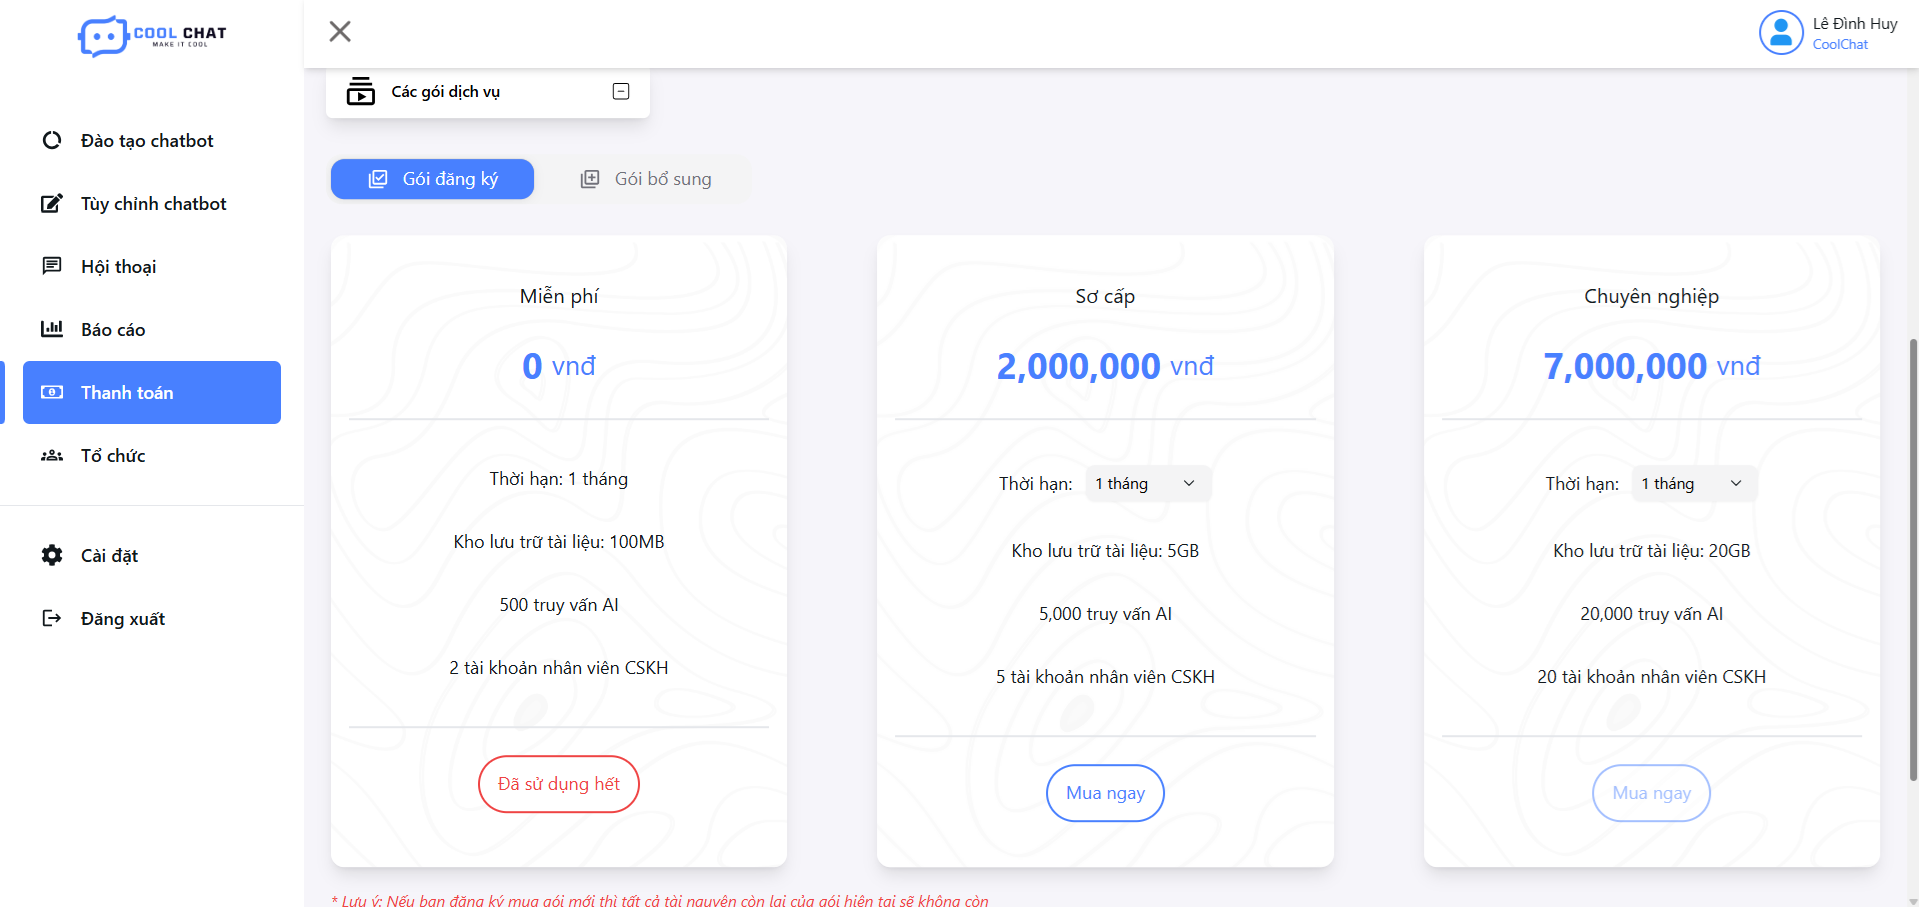
\includegraphics[width=1\textwidth]{Figma/sub_imple2.png}}
	\vspace{0.5cm}
	\caption{Các gói đăng ký}
	\label{fig:enter-label}
\end{figure}
\begin{figure}[H]
	\centering
	\fbox{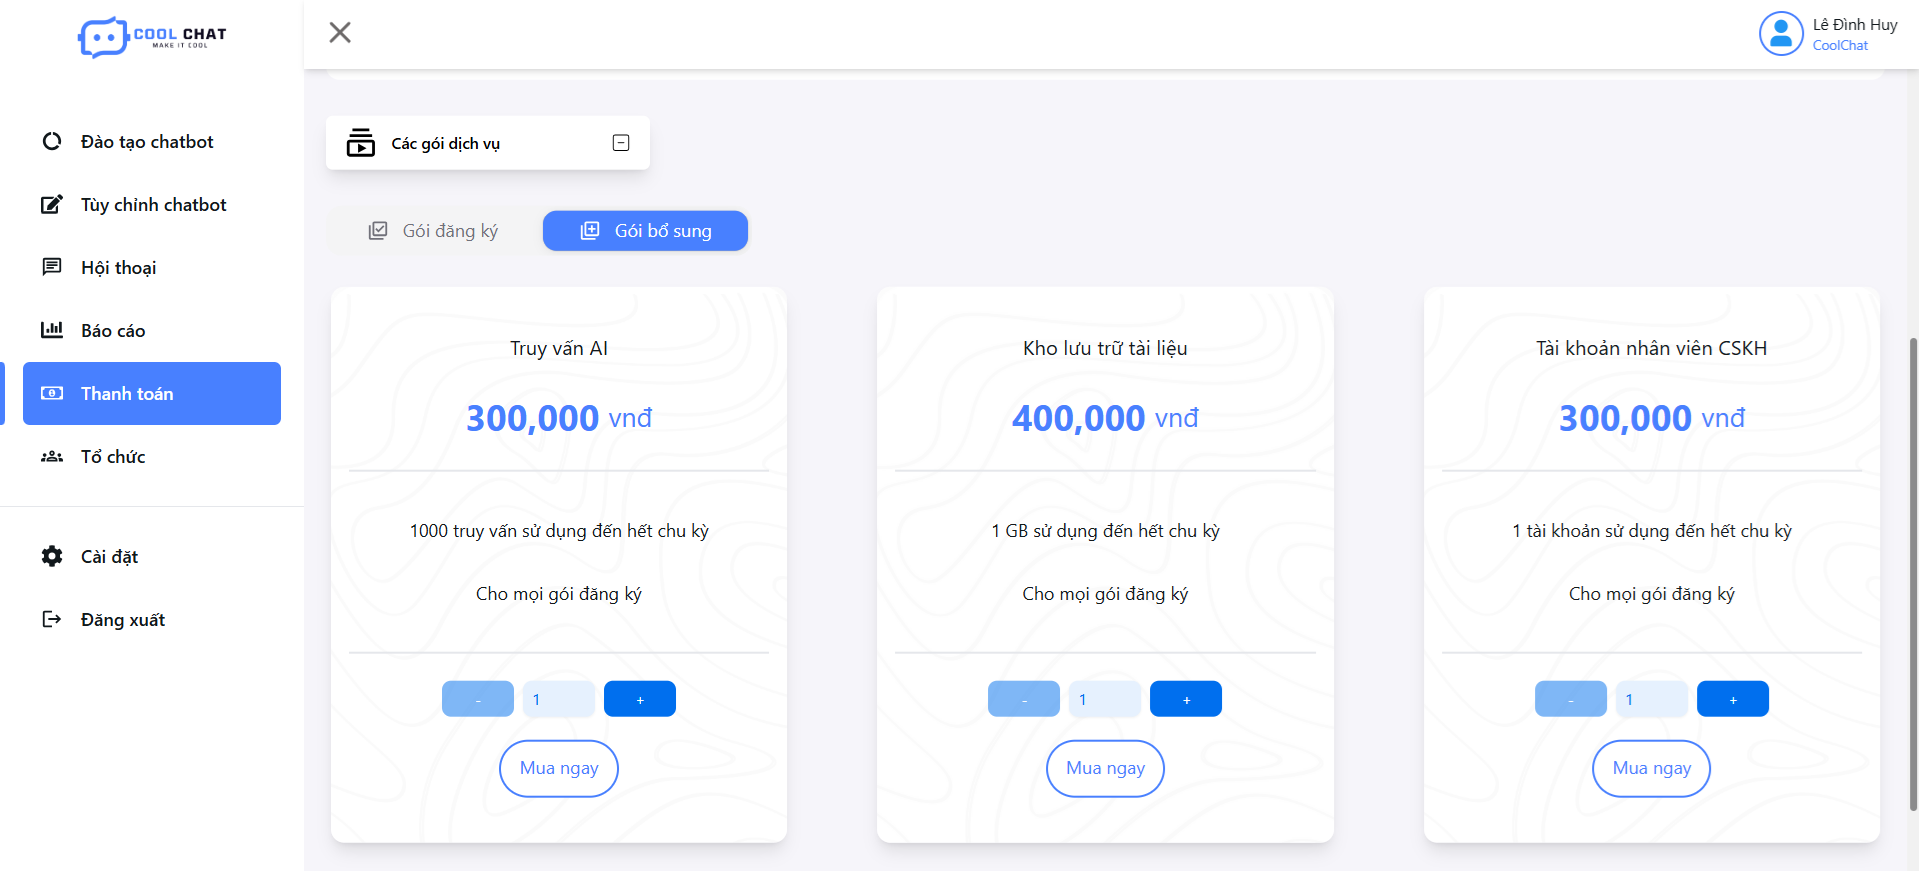
\includegraphics[width=1\textwidth]{Figma/sub_imple3.png}}
	\vspace{0.5cm}
	\caption{Các gói bổ sung}
	\label{fig:enter-label}
\end{figure}

Khi mua, hệ thống sẽ chuyển hướng đến trang thanh toán của PayOS như hình 95 chứa mã QR và các thông tin.
\begin{figure}[H]
	\centering
	\fbox{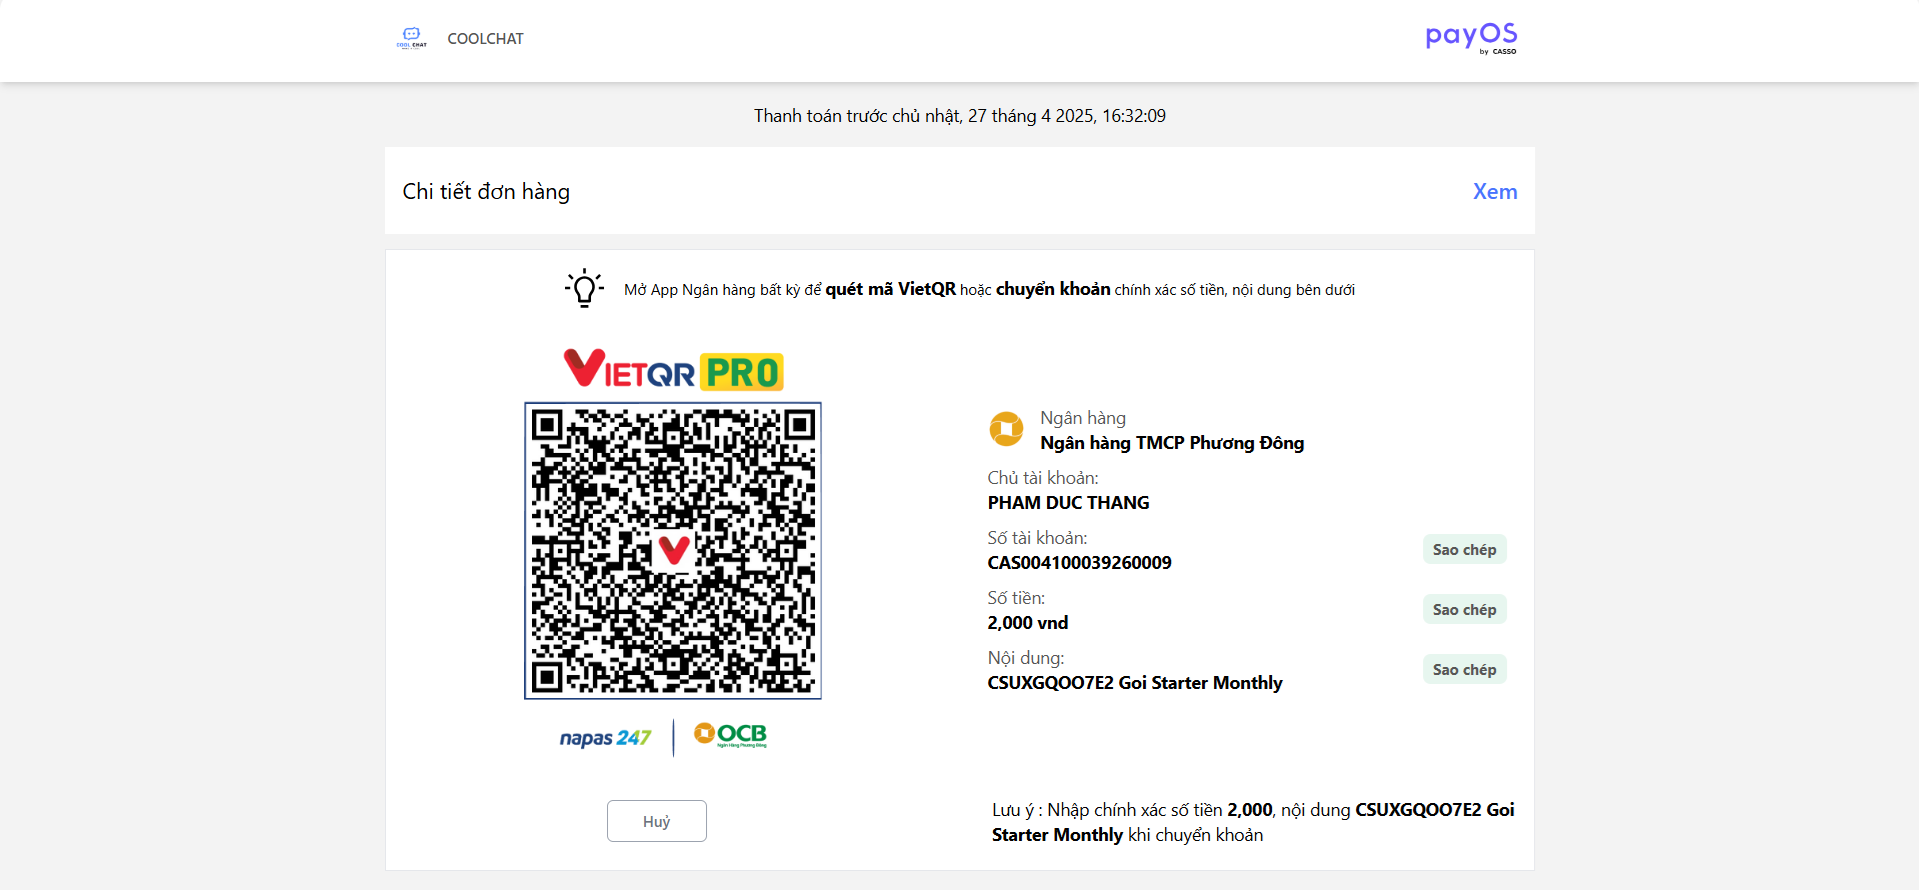
\includegraphics[width=1\textwidth]{Figma/sub_imple5.png}}
	\vspace{0.5cm}
	\caption{Giao diện thanh toán với PayOS}
	\label{fig:enter-label}
\end{figure}

Hệ thống còn hiển thị danh sách các lịch sử thanh toán  như hình 96 với các thông tin tương ứng, đối với hóa đơn ở trạng thái chờ, người dùng có thể tiếp tục thanh toán hoặc hủy gói.
\begin{figure}[H]
	\centering
	\fbox{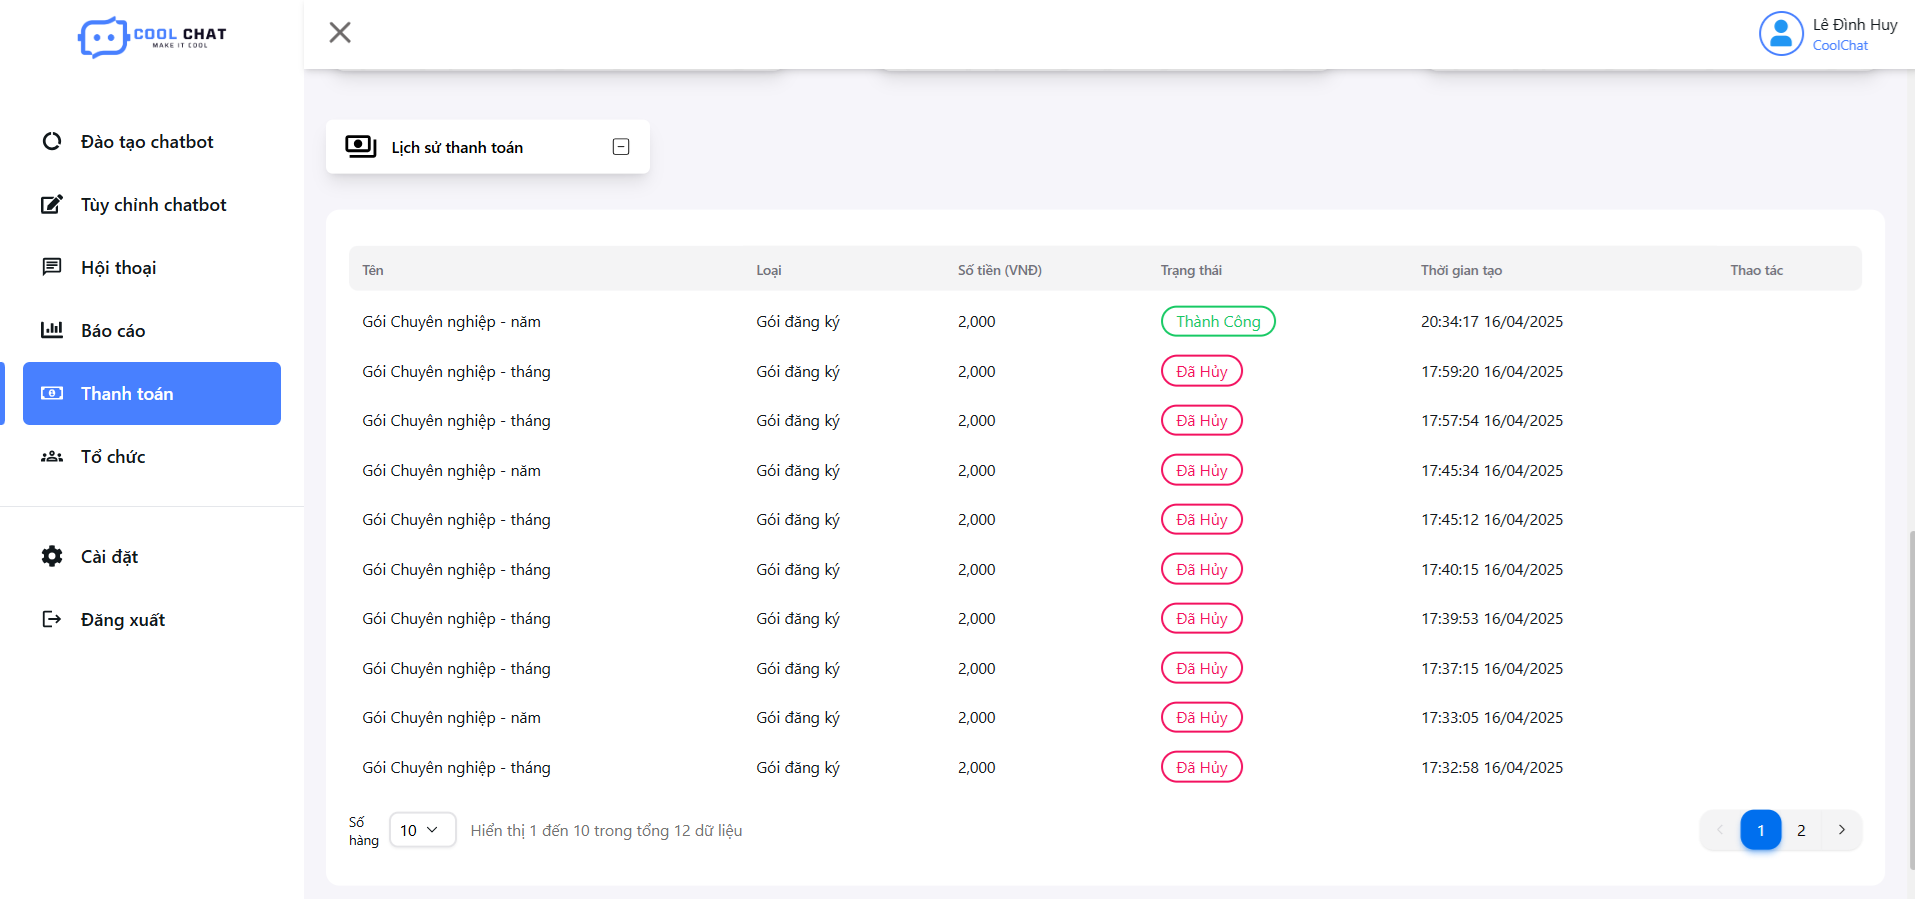
\includegraphics[width=1\textwidth]{Figma/sub_imple4.png}}
	\vspace{0.5cm}
	\caption{Giao diện thanh toán được hiện thực}
	\label{fig:enter-label}
\end{figure}
\subsubsection{Trang Tổ chức}
Trang tổ chức là trang cho phép quản lý tổ chức đối với chủ sở hữu tổ chức và chỉ hiển thị thông tin tổ chức đối với quản trị viên và nhân viên như hình 97. Chủ sở hữu có thể chỉnh sửa thông tin tổ chức, xem danh sách thành viên như hình 98, danh sách lời mời ở hình 99 và mời thêm thành viên vào tổ chức ở hình 100.
\begin{figure}[H]
	\centering
	\fbox{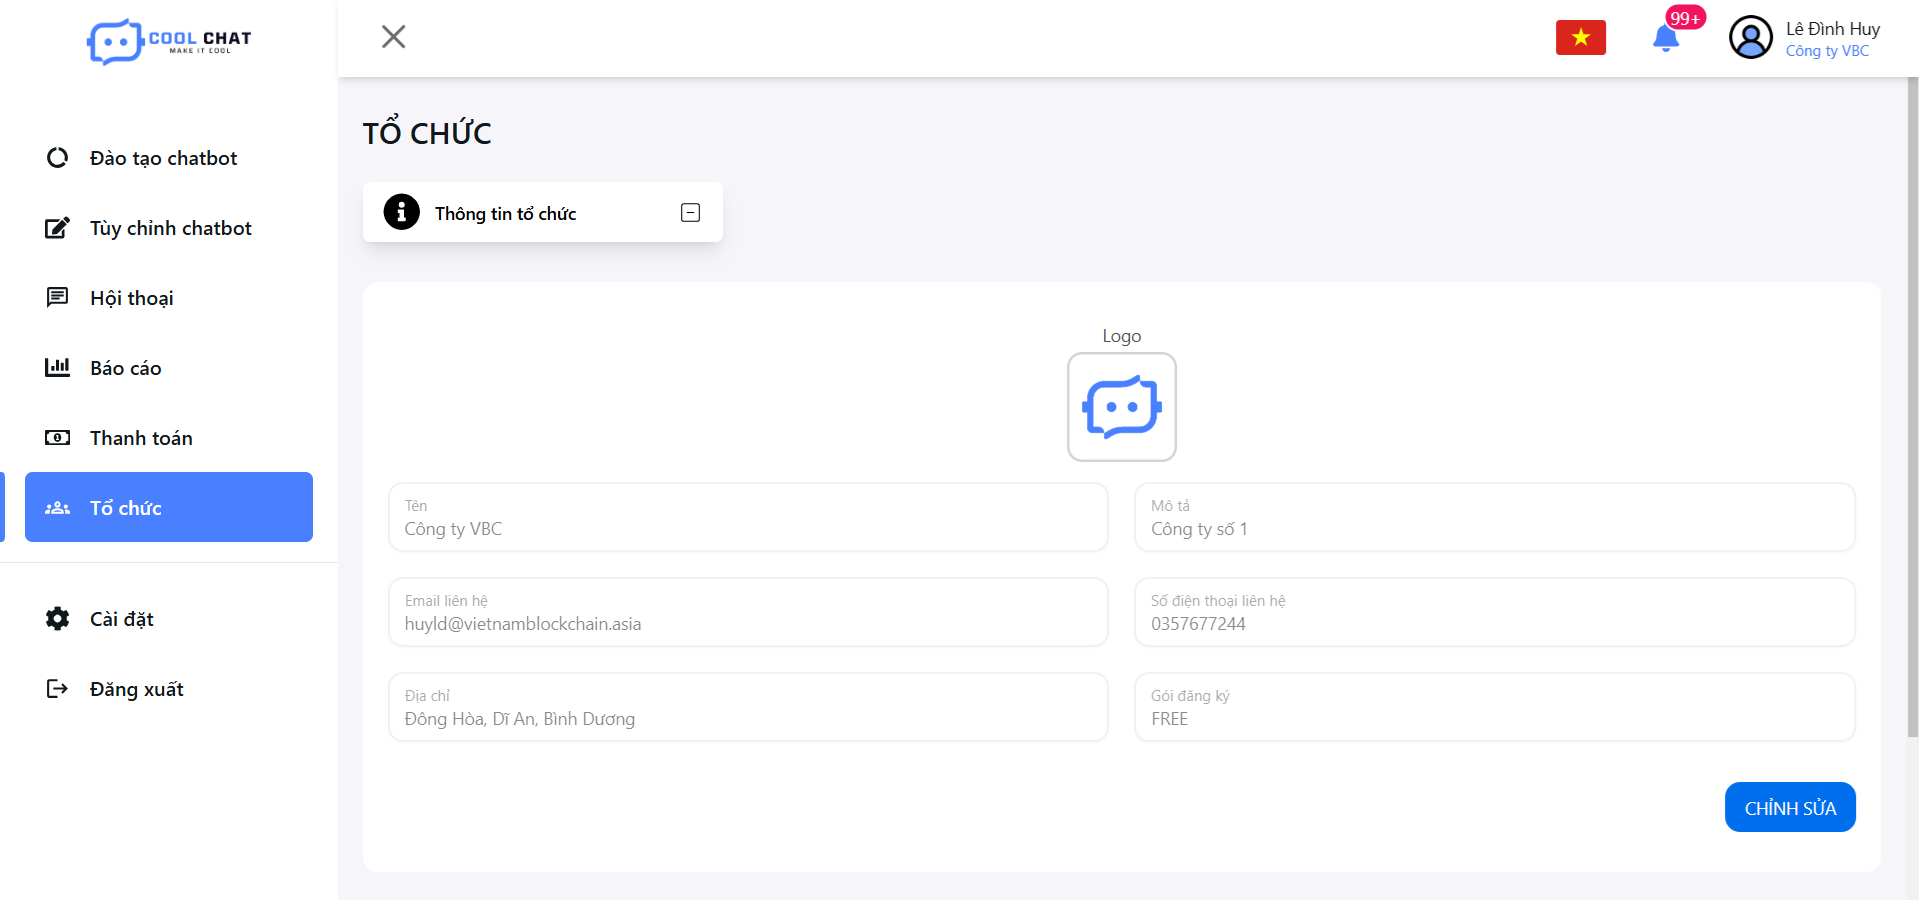
\includegraphics[width=1\textwidth]{Figma/org_1.png}}
	\vspace{0.5cm}
	\caption{Giao diện thông tin tổ chức}
	\label{fig:enter-label}
\end{figure}
\begin{figure}[H]
	\centering
	\fbox{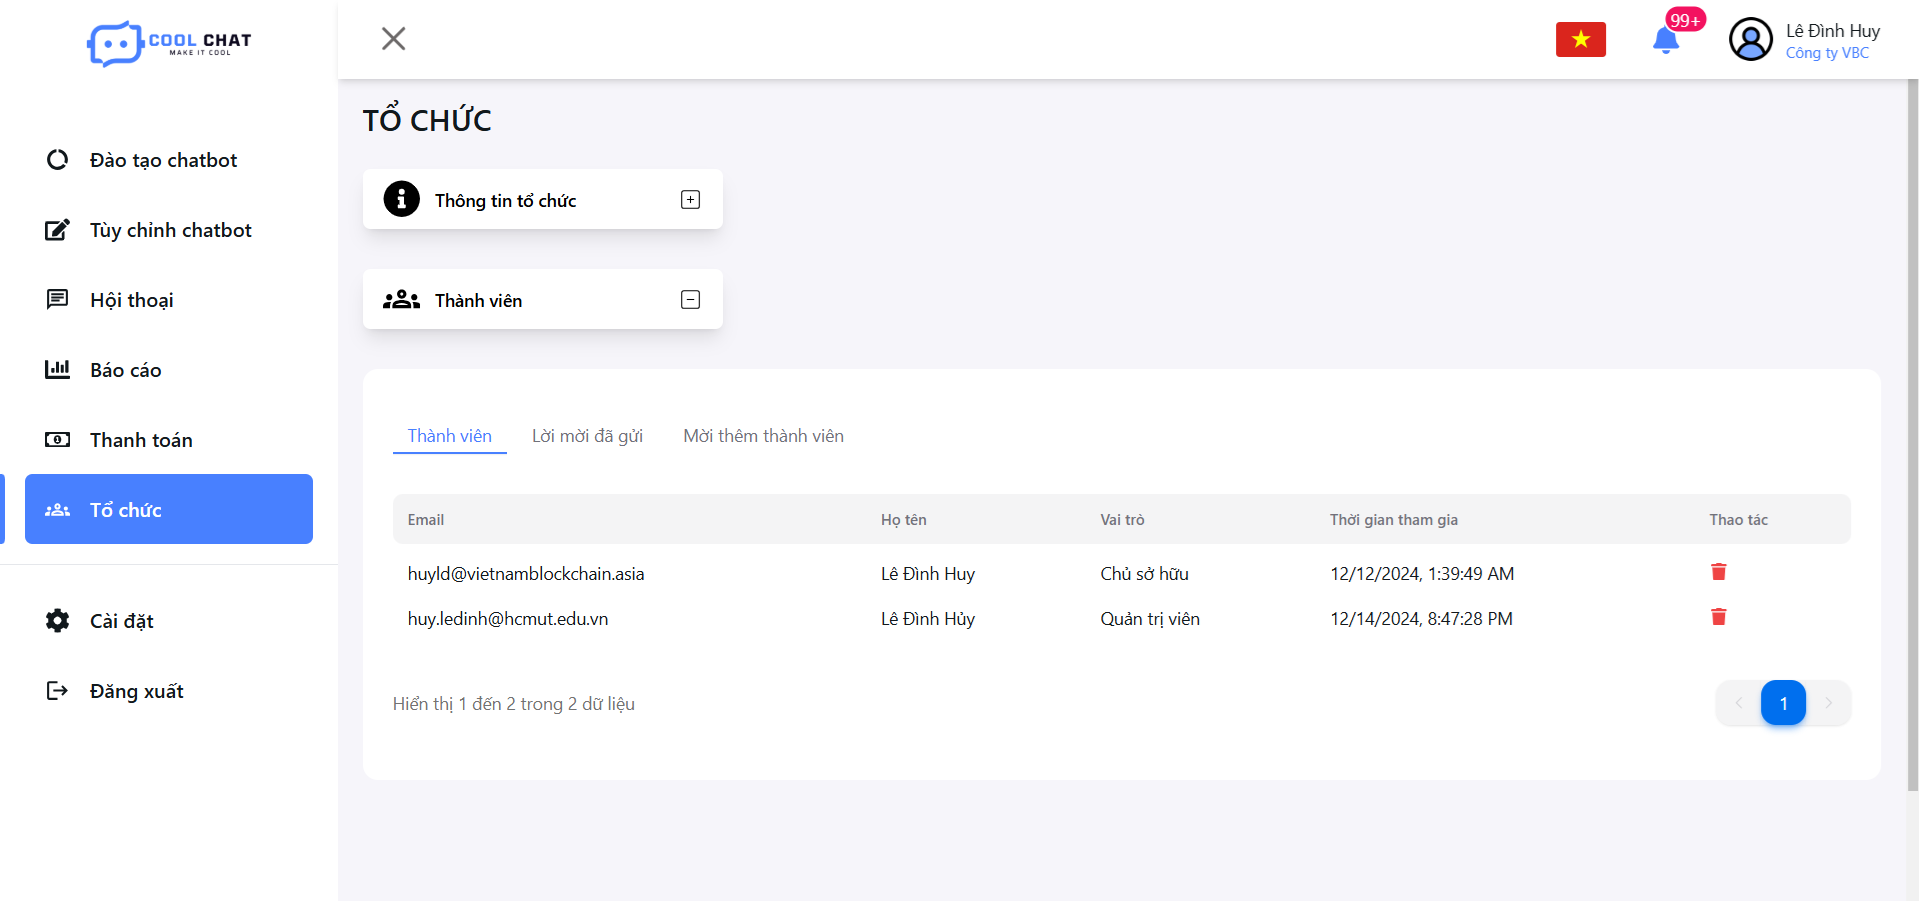
\includegraphics[width=1\textwidth]{Figma/org_3.png}}
	\vspace{0.5cm}
	\caption{Giao diện danh sách thành viên tổ chức}
	\label{fig:enter-label}
\end{figure}
\begin{figure}[H]
	\centering
	\fbox{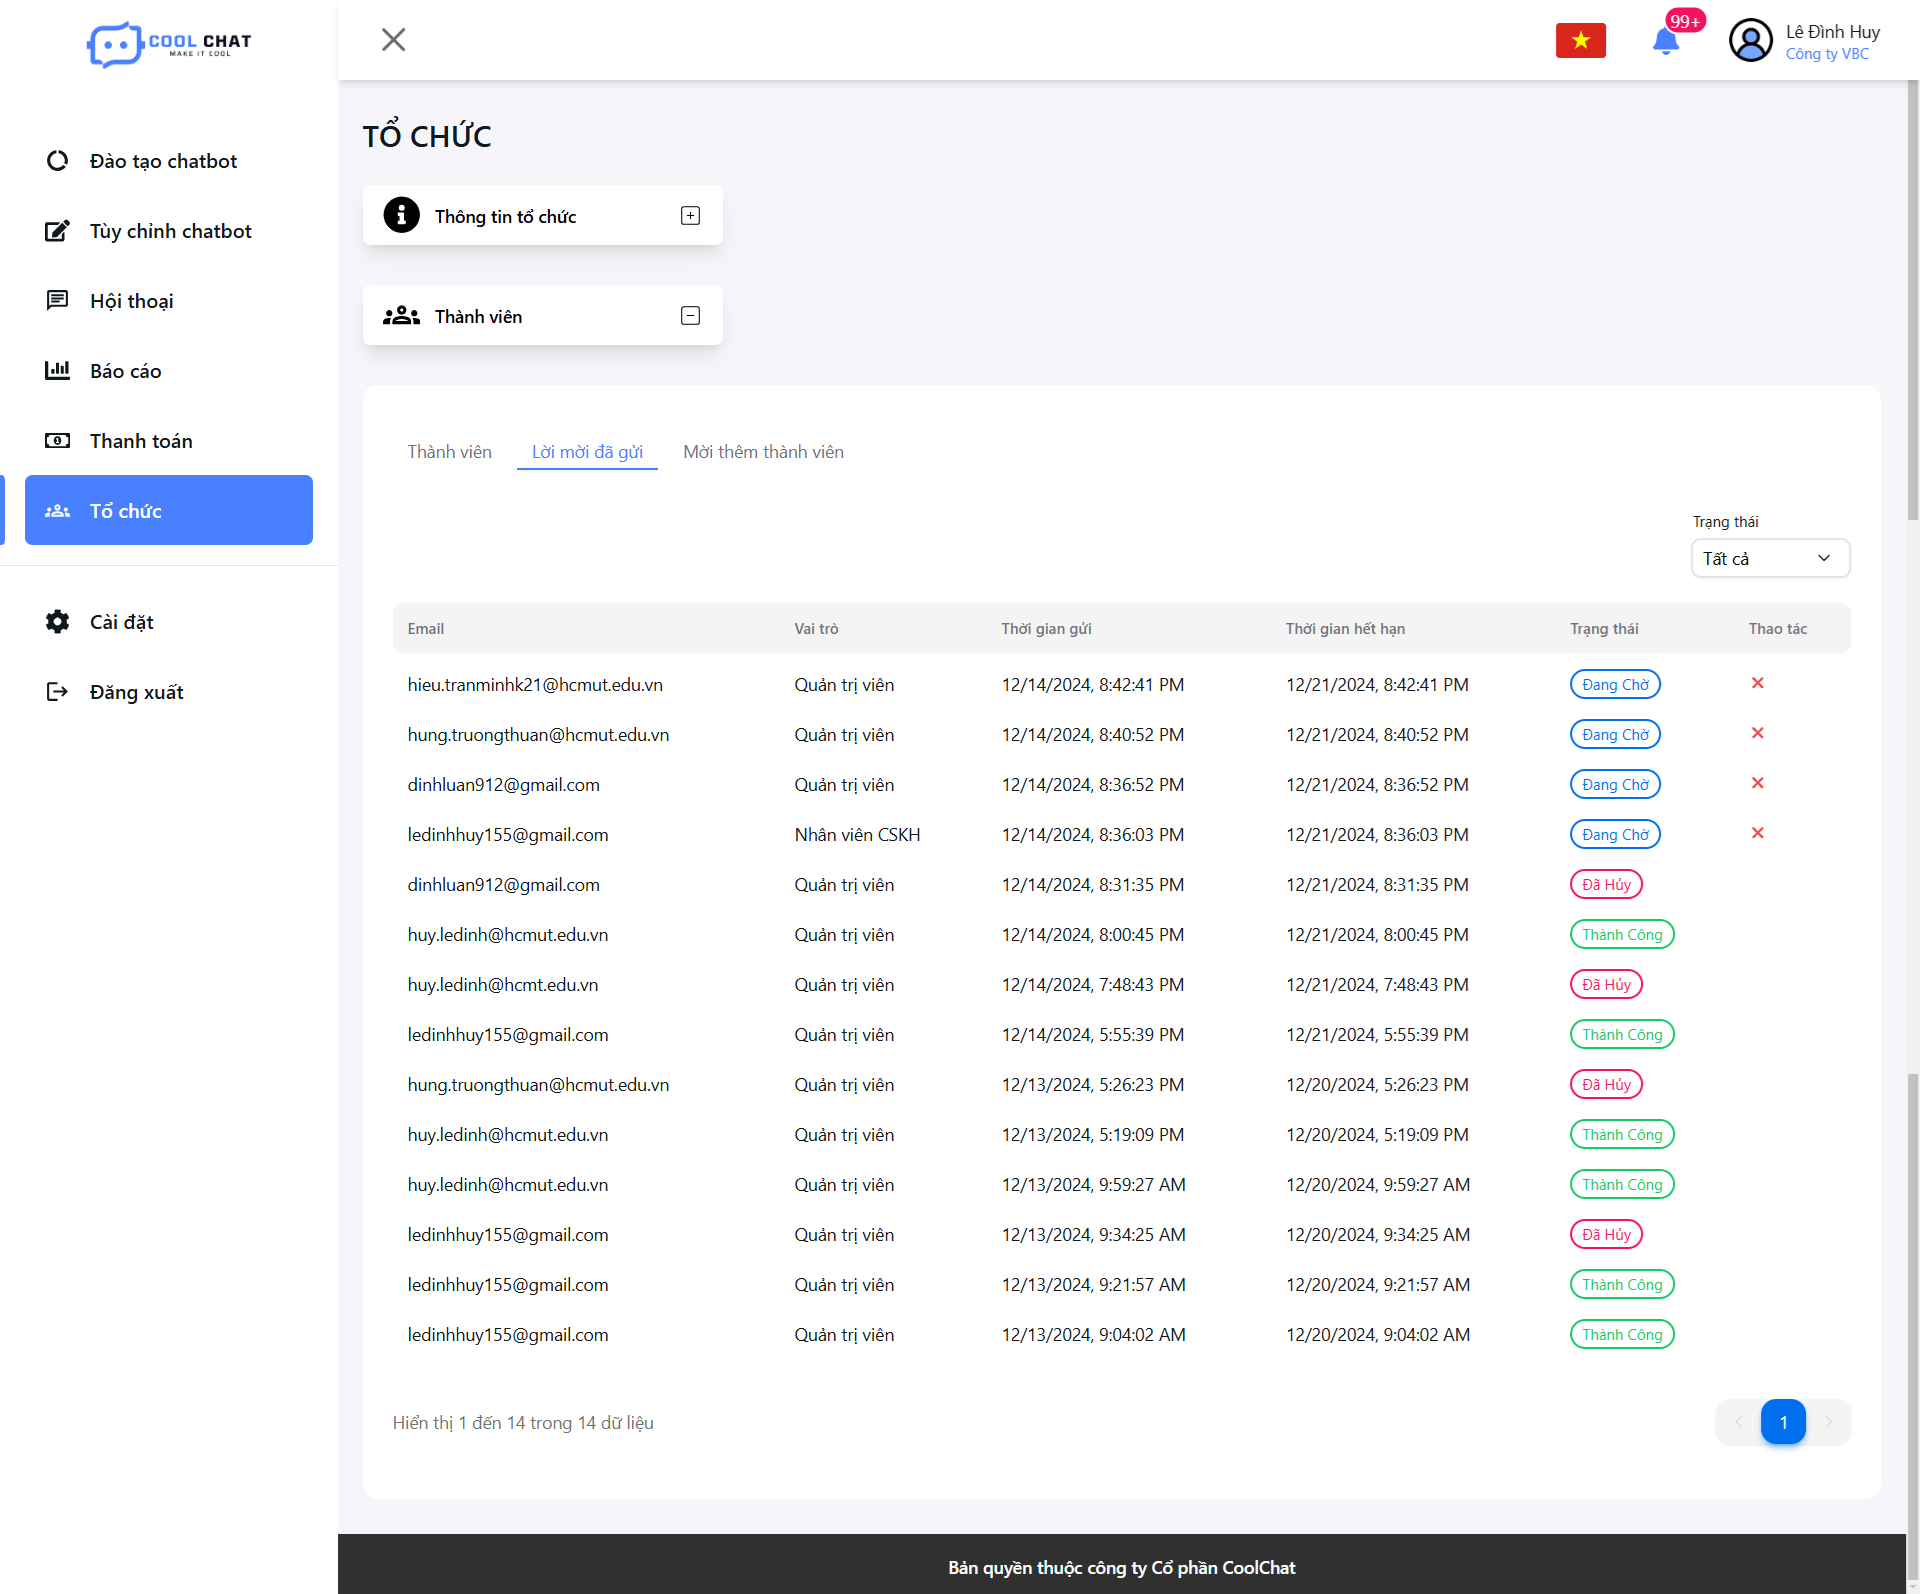
\includegraphics[width=1\textwidth]{Figma/org_4.png}}
	\vspace{0.5cm}
	\caption{Giao diện danh sách lời mời tham gia tổ chức}
	\label{fig:enter-label}
\end{figure}
\begin{figure}[H]
	\centering
	\fbox{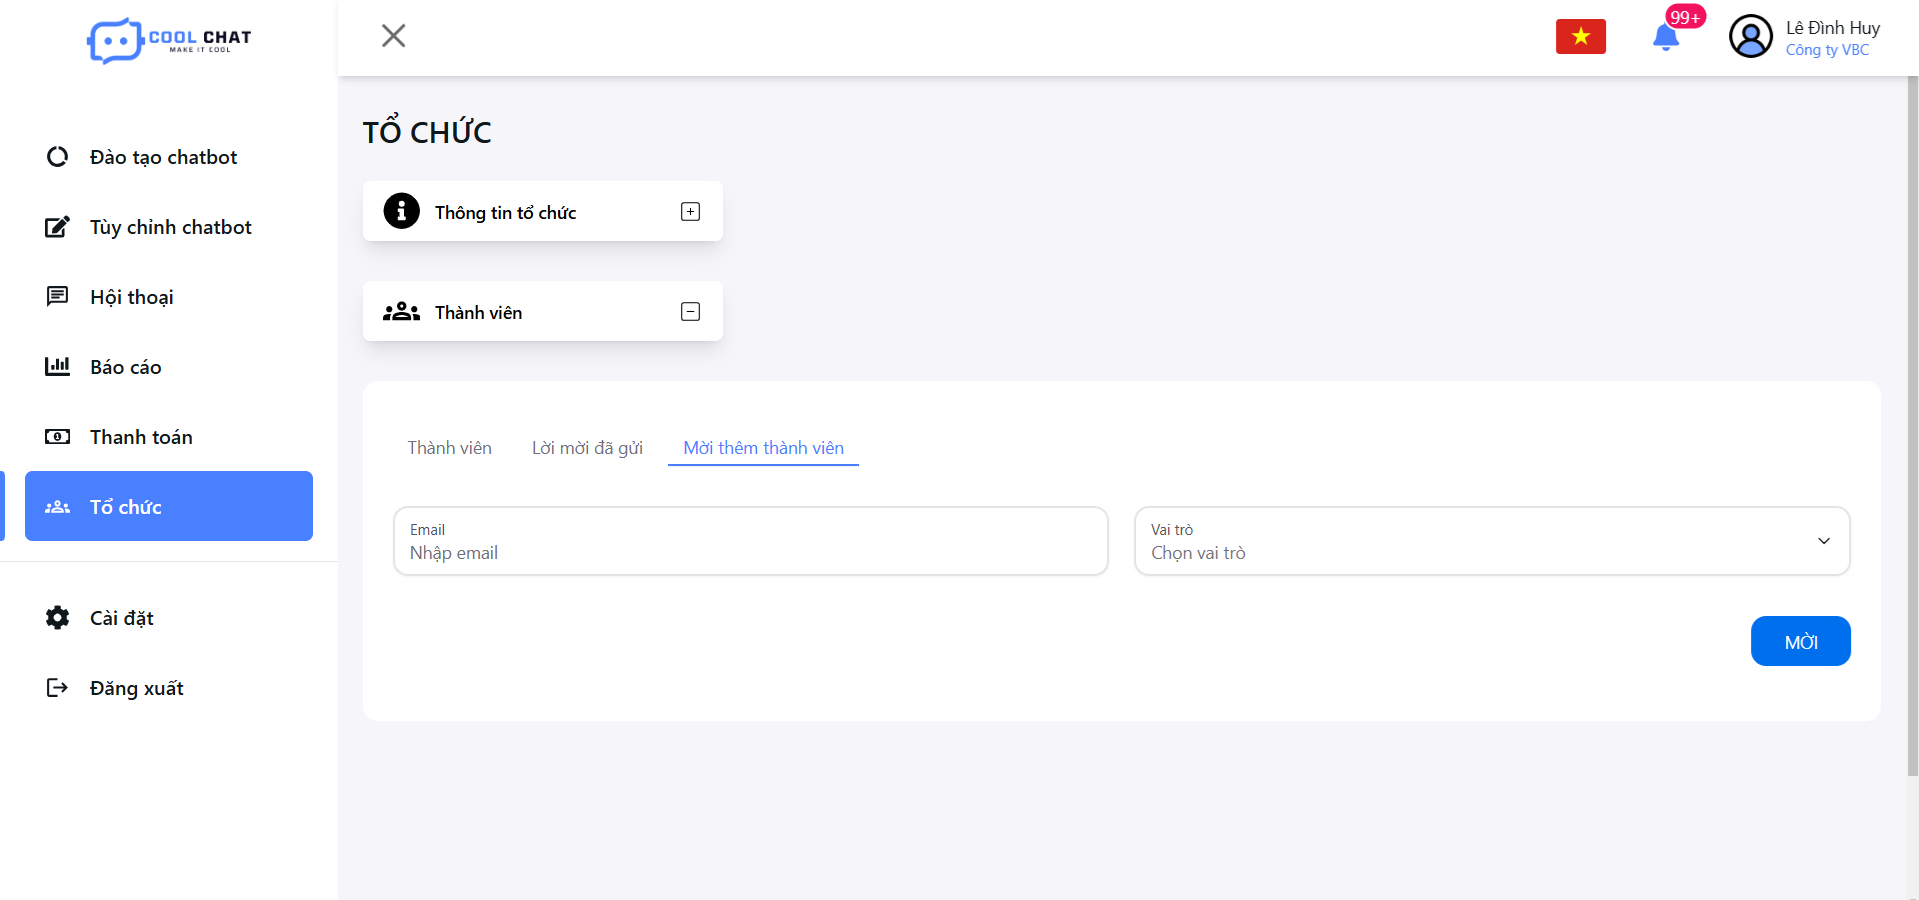
\includegraphics[width=1\textwidth]{Figma/org_5.png}}
	\vspace{0.5cm}
	\caption{Giao diện mời thêm thành viên vào tổ chức}
	\label{fig:enter-label}
\end{figure}

Khi chủ sở hữu điền thông tin và chọn gửi lời mời đến thành viên mới, thành viên mới sẽ nhận được một email tham gia tổ chức bao gồm các thông tin liên quan, mã giới thiệu và nút đăng ký dẫn đến trang đăng ký của hệ thống.

\subsubsection{Trang Cài đặt}
Mọi người dùng đều có thể chỉnh sửa thông tin cá nhân hoặc đổi mật khẩu ở trang Cài đặt như hình 101 và 102.
\begin{figure}[H]
	\centering
	\fbox{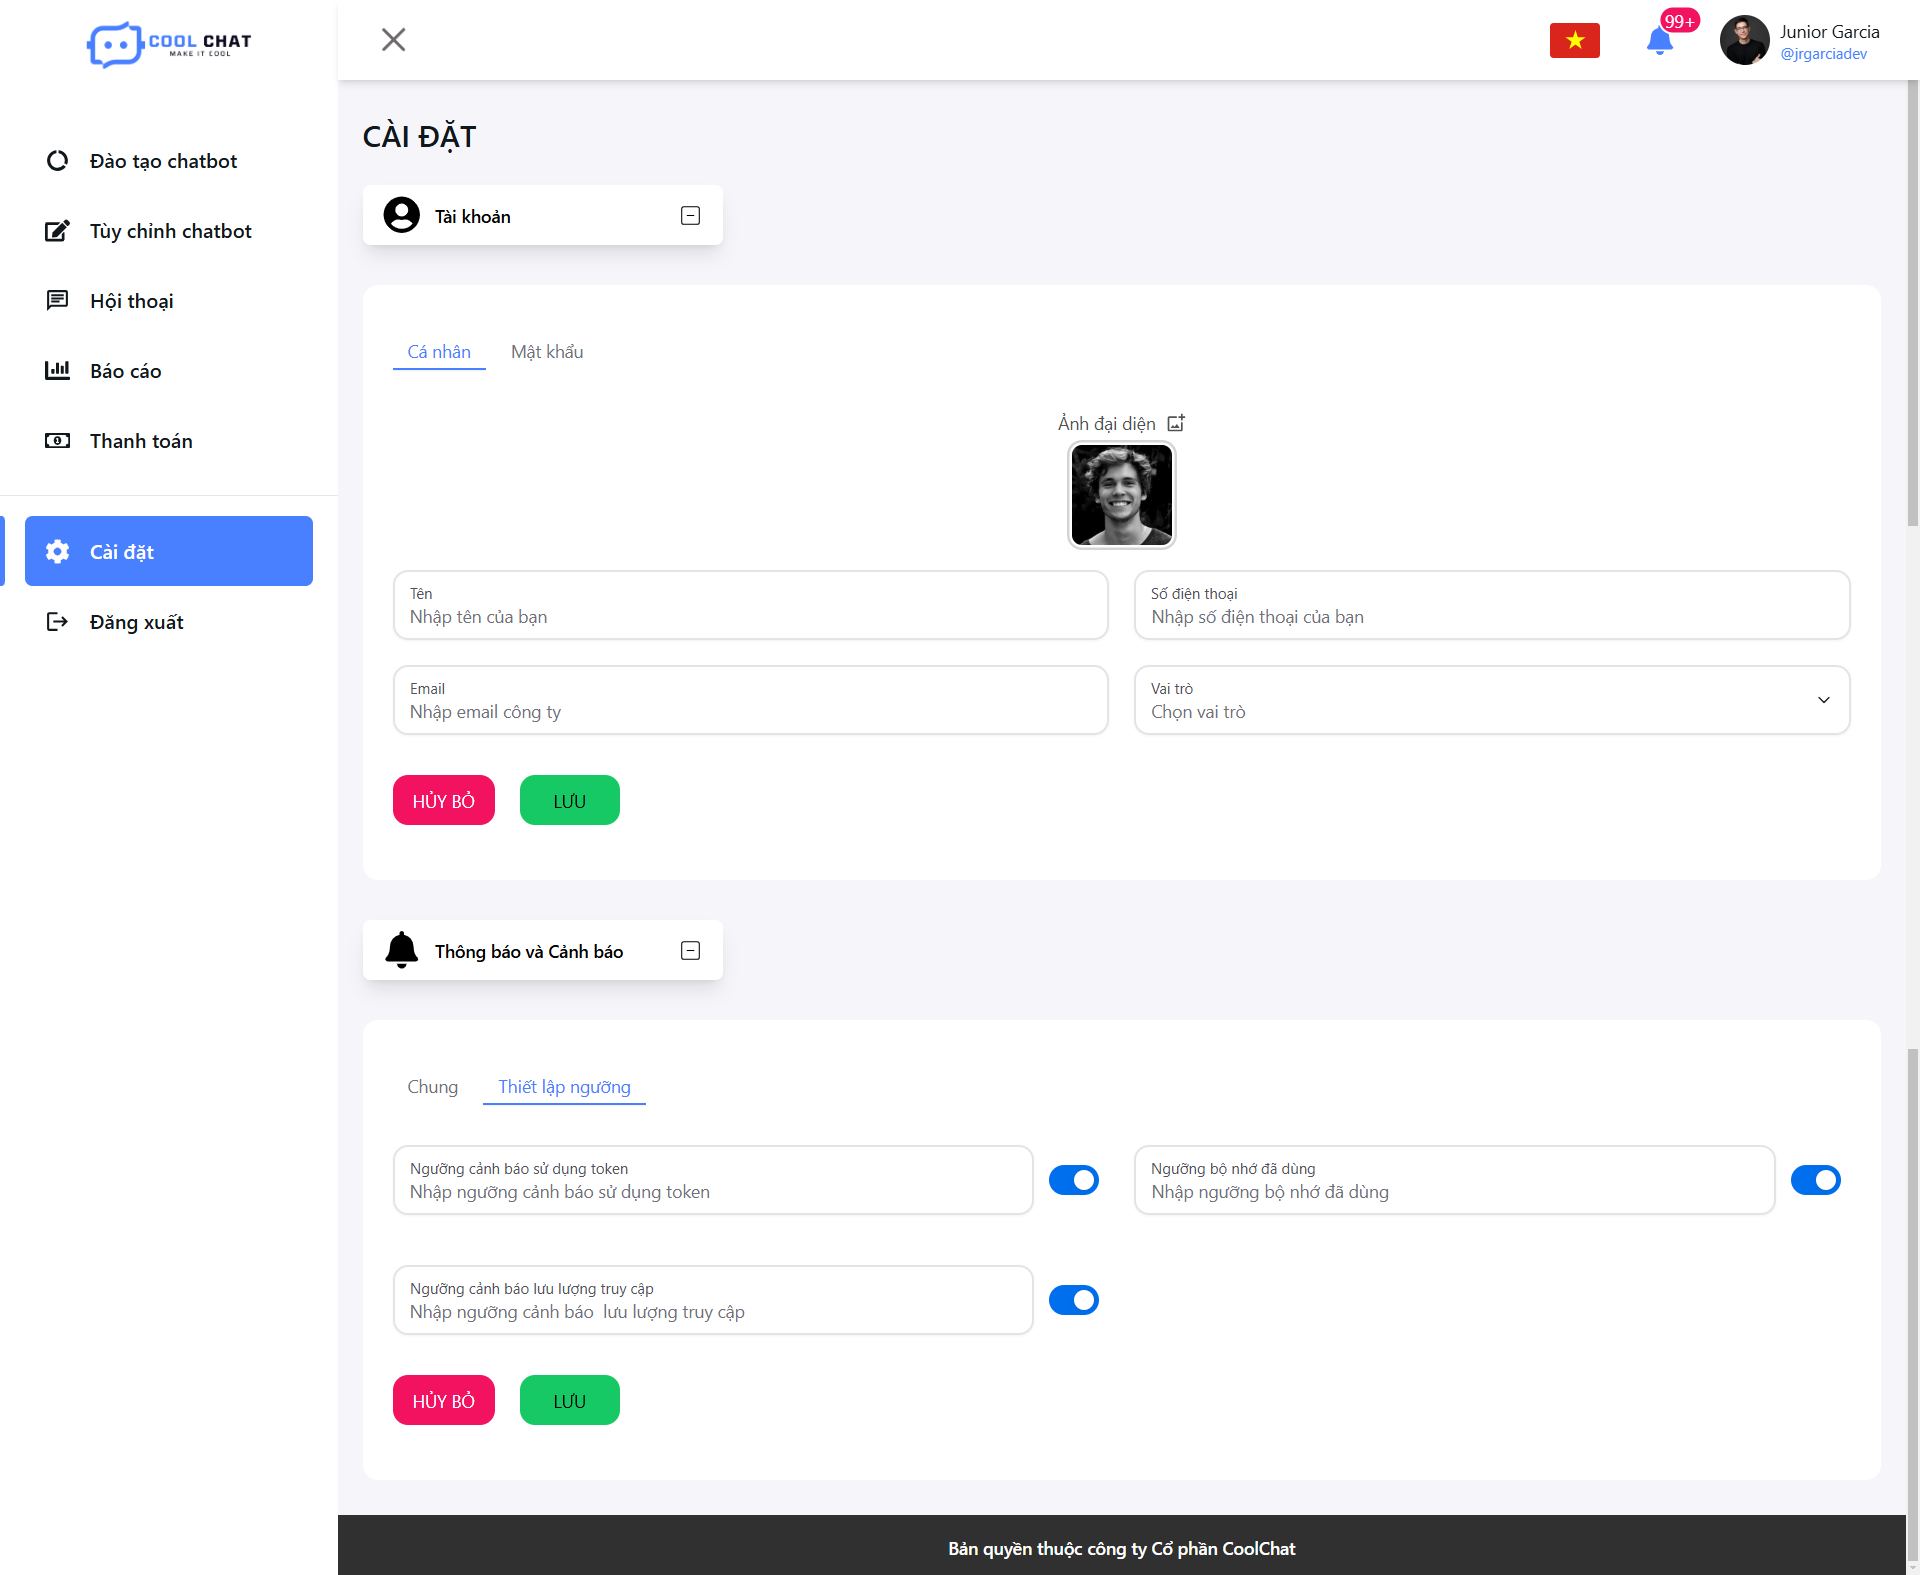
\includegraphics[width=1\textwidth]{Figma/setting_imple.png}}
	\vspace{0.5cm}
	\caption{Giao diện chỉnh sửa thông tin cá nhân}
	\label{fig:enter-label}
\end{figure}
\begin{figure}[H]
	\centering
	\fbox{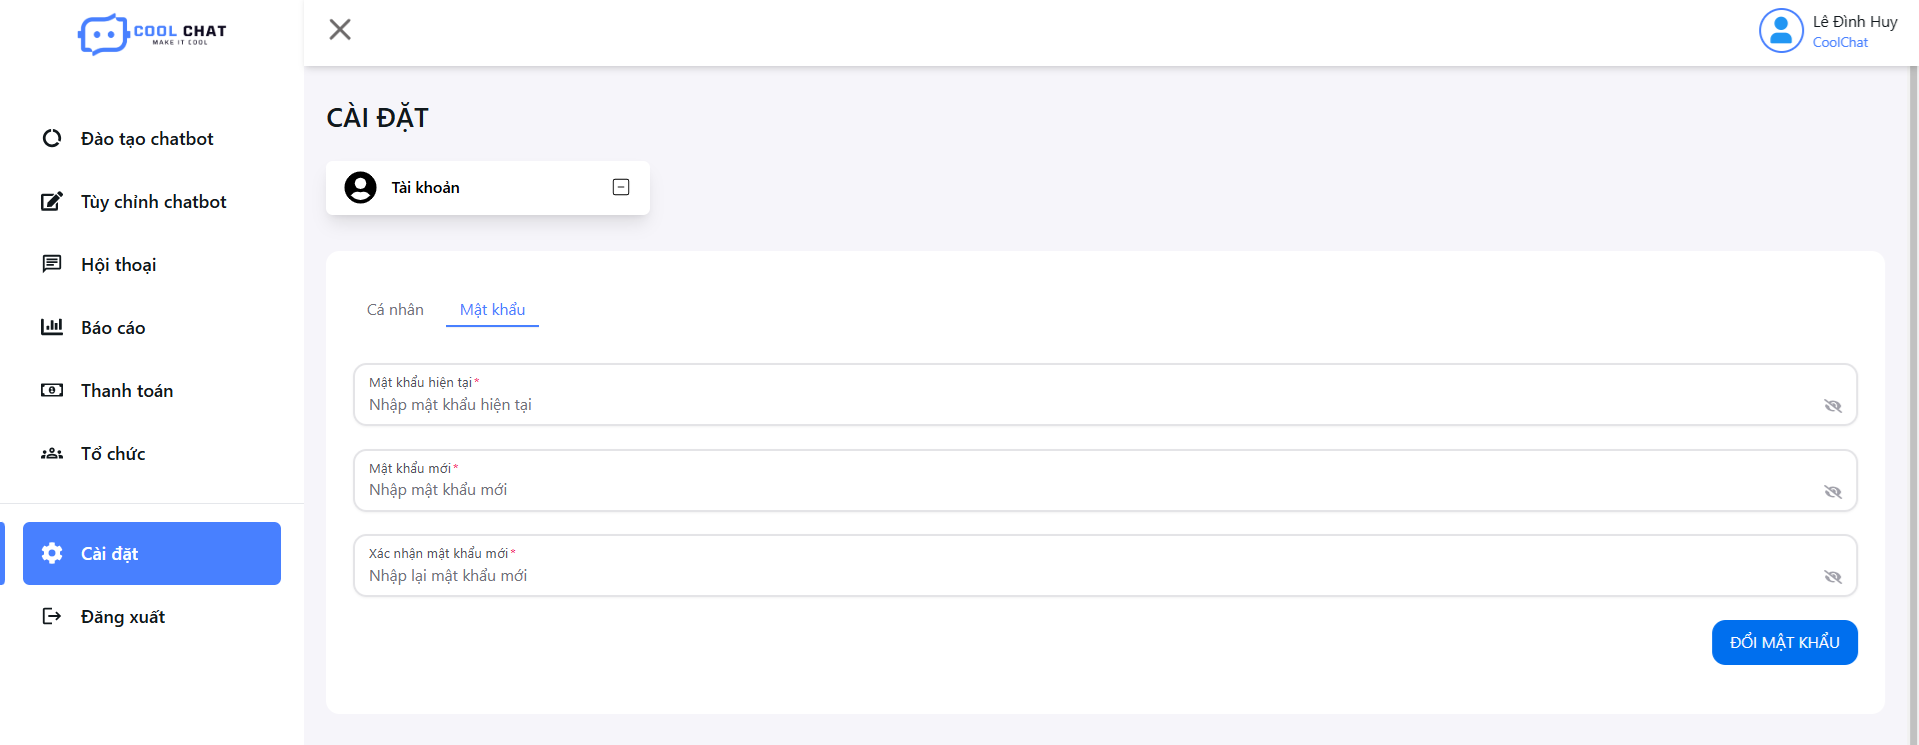
\includegraphics[width=1\textwidth]{Figma/setting_imple1.png}}
	\vspace{0.5cm}
	\caption{Giao diện đổi mật khẩu}
	\label{fig:enter-label}
\end{figure}

\subsubsection{Giao diện hộp chat dành cho khách hàng}
Mỗi hộp chat của mỗi tổ chức sẽ được tùy chỉnh khác nhau, tuy nhiên đều có những chức năng chung và bố cục giống nhau. Hình 103 cên dưới là giao diện bình thường được công ty CoolChat cấu hình và giao diện gửi yêu cầu hỗ trợ.
\begin{figure}[H]
	\centering
	\fbox{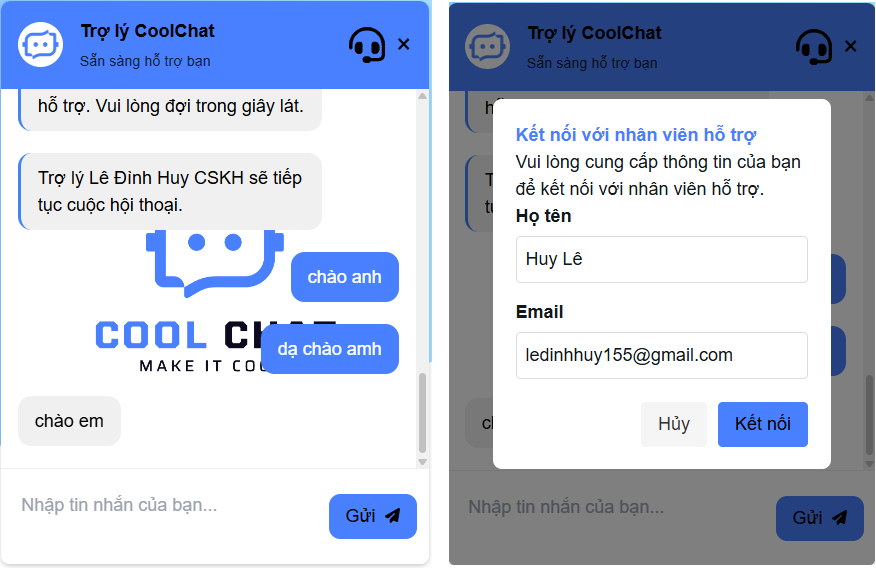
\includegraphics[width=0.8\textwidth]{Figma/chatbox_customewr.png}}
	\vspace{0.5cm}
	\caption{Giao diện chatbot phía khách hàng}
	\label{fig:enter-label}
\end{figure}

